\documentclass{article}

\usepackage[utf8]{inputenc}
\usepackage[russian]{babel}
\usepackage[a4paper, margin=1in]{geometry}
\usepackage{graphicx}
\usepackage{amsmath}
\usepackage{wrapfig}
\usepackage{multirow}
\usepackage{mathtools}
\usepackage{pgfplots}
\usepackage{pgfplotstable}
\usepackage{setspace}
\usepackage{changepage}
\usepackage{caption}
\usepackage{csquotes}
\usepackage{hyperref}
\usepackage{listings}

\pgfplotsset{compat=1.18}
\hypersetup{
  colorlinks = true,
  linkcolor  = blue,
  filecolor  = magenta,      
  urlcolor   = darkgray,
  pdftitle   = {
    semt-report-1-srs-smirnov-shinakov
  },
}

\begin{document}

\begin{titlepage}
  \begin{center}
    \begin{spacing}{1.4}
      \large{Университет ИТМО} \\
      \large{Факультет программной инженерии и компьютерной техники} \\
    \end{spacing}
    \vfill
    \textbf{
      \huge{Методы и средства программной инженерии.} \\
      \huge{Лабораторная работа №1.} \\
      \huge{Software Requirements Specification} \\
    }
  \end{center}
  \vfill
  \begin{center}
    \begin{tabular}{r l}
      Смирнов Виктор Игоревич  & P32131 \\
      Шиняков Артём Дмитриевич & R32372 \\
      Вариант                  & 1025   \\
    \end{tabular}
  \end{center}
  \vfill
  \begin{center}
    \begin{large}
      2023
    \end{large}
  \end{center}
\end{titlepage}

\tableofcontents

\section{Введение}

\subsection{Цель}
[Specify the purpose of this SRS. The SRS should 
fully describe the external behavior of the 
application or subsystem identified. It also 
describes nonfunctional requirements, design 
constraints and other factors necessary to 
provide a complete and comprehensive description 
of the requirements for the software.]

Документ представляет из себяс процесс и требования 
к разработке сайта для международного
аэропорта Домодедово, расположенного в 
городе Москва. Требования к сайту описаны ниже.


\subsection{Краткая сводка возможностей}
[A brief description of the software application 
that the SRS applies to; the feature or other 
subsystem grouping; what Use-Case model(s) it 
is associated with;  and anything else that is 
affected or influenced by this document.]

Работающий сайт, предоставляющий информацию о состоянии аэропорта и рейсов, у которых одним из пунктов назначения/вылета указан Домодедово, 
новости, касающиеся данного аэроузла, возможность бронирования билетов на перелеты, план местности для ориентации пассажиров,
подробные указания пути до Домодедово, сведения о доступных поблизости местах отдыха/ночлега, юридические документы, содержащие описание 
прав и обязанностей пассажиров и посетителей, а также способы связи с представителями данной организации.
Взаимодействие с клиентом осуществляется 2 способами: 
1)Клиент связывается с компанией через контакты или социальные, указанные на сайте
2)Клиент бронирует места на рейс или в гостинице, указывая свои персональные данные
Сервер должен поддерживать роботоспособность сайта, транзакции при оплате билетов и предоставлять актуальную информацию о состоянии полетов.

\subsection{Определения, акронимы и сокращения}
% [This subsection should provide the definitions 
% of all terms, acronyms, and abbreviations required 
% to properly interpret the SRS.  This information 
% may be provided by reference to the project 
% Glossary.]

\begin{itemize}
    \item Посетитель или пассажир - любой человек, зашедший на сайт
    \item Личный кабинет - страница, которая отображает информацию о каждом зарегистрированном пользователе.
    \item Администратор - сотрудник аэропорта Домодедово или смежных компаний, имеющий свой личный кабинет и обладающий определенными правами,
    недоступными обычным посетителям.
    \item Интеграция - использование систем компаний-представителей платежных систем и сотрудничество с ними.
    \item Платёжная система - сервис, предоставляющий возможность перевода денег между двумя счетами.
    \item Раздел сайта - отдельная страница(возможно с ссылками на другие)
    \item База данных - упорядоченный набор структурированной информации или данных, которые обычно хранятся в электронном виде в компьютерной системе.
    \item Информационная страница - страница сайта, содержащая только текстовую и ссылочную информацию в качестве основного содержания.
    \item Титульная страница - страница, на которую попадает изначально пользователь.
    \item Согласованность данных - целостность данных, а также внутренняя непротиворечивость.
\end{itemize}

\subsection{Ссылки}

\begin{itemize}
    \item Редактор Use-case диаграмм:
          \url{https://creately.com/diagram-type/use-case/}
    \item SRS шаблон:
          \url{https://docs.google.com/document/d/11aTUhjJxHqDMJGTDXDKh_8U_f2YVWKBS/edit?usp=sharing&ouid=112239579841283566048&rtpof=true&sd=true}
\end{itemize}


\subsection{Обзор}

Документ разделен на части, осписанные ниже
\begin{enumerate}
      \item \textbf{Введение} \\
            Содержит общие сведения о документе. Описывает
            используемые ресурсы и определения.

      \item \textbf{Общее описание} \\
            Раздел содержит обобщенное описание проекта,
            аудитории, ограничений и подводных камней.

      \item \textbf{Требования} \\
            Раздел описывает все требования, предъявляемые
            разрабатываемой системе. Все упомянутые требования
            должны быть соблюдены.

      \item \textbf{Use-Case} \\
            Раздел описывает возможные сценарии взаимодействия
            пользователя и разрабатываемого рещения.

      \item \textbf{UML-диаграмма} \\
            Раздел состоит из UML-диаграммы, графически
            описывающей архитектуру и реализацию программной
            системы.
\end{enumerate}


\section{Общее описание}

\subsection{Функционал продукта}
Cайт должен давать возможность отслеживания 
всех грузовых и пассажирских рейсов вылетающих из/прибывающих в 
аэропорт Домодедово, поиска полетов по их 
параметрам и атрибутам, прочтения новостей, 
связанных с аэропортом, отслеживания состояния 
аэропорта, услуг и возможностей, которые он предоставляет. 
Также разрабатываемое решение должно предоставлять 
услугу бронирования и приобретения авиабилетов, 
отображения избранных рейсов клиента, отображение плана территории, 
возможность бронирования номеров в отелях и гостиницах города Москва, 
покупка парковочного места для авторизованных пользователей,
возможные маршруты до аэропорта и обратную 
связь с представителями Домодедово.


\subsection{Описание пользователей}

\begin{enumerate}
      \item Клиенты, обладающие необходимостью в
            приобретении билета или отслеживании состояния 
            определенного рейса
            
      \item Пассажиры, желающие забронировать место
            проживания или парковочное пространство по 
            прибытии или заранее
            
      \item Администраторы и работники аэропорта
            Домодедово
            
      \item Представители компаний авиаперевозок,
            пользующиеся пространством аэропорта
\end{enumerate}


\subsection{Факторы и зависимости}
TODO: here we should describe what we need to launch our project

Для реализации транзакций необходимо подключиться к одной из популярных платежных систем.\\
Для отображения актуального расписания и состояния полетов необходимо соединение с базами данных авиакомпаний, 
обслуживаемых аэропортом Домодедово.

\subsection{Ограничения}
\begin{itemize}
      \item На разрабатываемый сайт накладываются
            ограничения изложенные в этом файле.
            
      \item Незадокументированные требования не
            учитываются при создании технического 
            решения задач.
            
      \item Ограничениями на минимальный функционал сайта
            являются требования из раздела функциональных.
            
      \item Ограниениями на используемые технологии
            являются требования из раздела нефункциональных.
\end{itemize}

% TODO: после нефункциональных посмотрим, мб допишем.


\section{Технические требования}

\subsection{Функциональность}
Примечание: 1sp = 24 часа.
\begin{enumerate}
      \item Система должна позволять пользователю просматривать
            табло с расписанием полетов, начальным или конечным
            пунктом которых указан аэропорт Домодедово. \\
            Приоритет: Высокий. Стабильность: Высокая. Трудоёмкость: 10 sp.

      \item Система должна содержать онлайн табло, отображающее расписание рейсов,
            должно иметь функцию поиска по номеру рейса/направлению полета. \\
            Приоритет: Высокий. Стабильность: Средняя. Трудоёмкость: 6 sp.

      \item Система должна содержать страницу с новостями, которая должна
            предусматривать функцию фильтрации по дате публикаций и по
            теме новостных записей. \\
            Приоритет: Высокий. Стабильность: Средняя. Трудоёмкость: 12 sp.

      \item Система должна содержать контакты для связи с
            представителями аэропорта Домодедово и ссылки
            на страницы в социальных сетях. \\
            Приоритет: Высокий. Стабильность: Средняя. Трудоёмкость: 2 sp.

      \item Система должна предоставлять администраторам
            доступ к базе данных клиентов сервиса
            PARKING.DME.RU. \\
            Приоритет: Высокий. Стабильность: Средняя. Трудоёмкость: 10 sp.

      \item Система должна предоставлять администратором возможность
            добавления новых новостей в ленту. \\
            Приоритет: Высокий. Стабильность: Средняя. Трудоёмкость: 10 sp.

      \item Система должна давать администраторам возможность
            создавать и удалять экстренные/временные
            оповещения об изменениях в работе аэропорта. \\
            Приоритет: Высокий. Стабильность: Высокая. Трудоёмкость: 8 sp.

      \item Система должна давать администраторам возможность
            отслеживания заполненных форм обратной связи. \\
            Приоритет: Средний. Стабильность: Низкая. Трудоёмкость: 8 sp.

      \item Система должна отображать пользователю оповещения о
            срочных/временных изменениях работы аэропорта
            Домодедово на главной странице сайта. \\
            Приоритет: Высокий. Стабильность: Высокая. Трудоёмкость: 8 sp.

      \item Система должна отображать пользователю ленту
            новостей, связанных с аэропортом Домодедово. \\
            Приоритет: Высокий. Стабильность: Средняя. Трудоёмкость: 5 sp.

      \item Система должна предоставлять пользователям возможность заполнения
            и отправки формы обратной связи. \\
            Приоритет: Низкий. Стабильность: Средняя. Трудоёмкость: 8 sp.

      \item Система должна предоставлять пользователю возможность поиска
            и отслеживания рейсов по пункту назначения,
            авиакомпании, предоставляющей услуги, или
            направлению, и дате отправления. \\
            Приоритет: Высокий. Стабильность: Высокая. Трудоёмкость: 8 sp.

      \item Система должна предоставлять пользователю возможность бронирования
            и покупки авиабилетов на рейсы, имеющие
            свободные места. \\
            Приоритет: Высокий. Стабильность: Средняя. Трудоёмкость: 30 sp.

      \item Система должна предоставлять пользователю
            регистрации личного кабинета партнера или
            пассажира. Для пассажиров долен быть
            огранизован доступ к бронировнаию парковочных
            мест на сайте PARKING.DME.RU. Для партнеров
            доступны модули для работы с cargo. \\
            Приоритет: Средний. Стабильность: Средняя. Трудоёмкость: 14 sp.

      \item Система должна предоставлять пользователю возможность
            отслеживания груза по его накладному номеру. \\
            Приоритет: Высокий. Стабильность: Средняя. Трудоёмкость: 10 sp.

      \item Система должна предоставлять пользователю возможность
            заполнения и отправки анкеты соискателя. \\
            Приоритет: Низкий. Стабильность: Низкая. Трудоёмкость: 8 sp.

      \item Система должна предоставлять пользователю возможность
            просмотра юридических документов, определяющих
            условия работы аэропорта и пердоставления
            услуг авиакомпаниями. \\
            Приоритет: Низкий. Стабильность: Низкая. Трудоёмкость: 5 sp.

      \item Система должна предоставлять пользователю возможность просмотра
            информационных страниц с описанием услуг и
            условий пользования аэропортом. Также должна
            предоставляться возможность печати отдельных
            страниц. \\
            Приоритет: Средний. Стабильность: Низкая. Трудоёмкость: 5 sp.

\end{enumerate}


\subsection{Требования}

\begin{enumerate}
    \item Разрабатываемый раздел сайта должен позволять пользователю
          просматривать табло с расписанием полетов, начальным или
          конечным пунктом которых указан аэропорт Домодедово. \\
          Трудоёмкость: 8. Риск: Средний. Приоритет: Высокий.
    \item Онлайн табло, отображающее расписание рейсов должно иметь
          функцию поиска по номеру рейса/направлению полета. \\
          Трудоёмкость: 8. Риск: Средний. Приоритет: Высокий.
    \item Онлайн табло, отображающее расписание рейсов должно иметь
          функцию поиска по номеру рейса/направлению полета. \\
          Трудоёмкость: 8. Риск: Средний. Приоритет: Высокий.
    \item Страница с новостями должна предусматривать функцию
          фильтрации по дате публикаций и по теме новостных записей. \\
          Трудоёмкость: 8. Риск: Низкий. Приоритет: Средний.
    \item Сайт должен содержать контакты для связи с представителями
          аэропорта Домодедово и ссылки на социальные контакты \\
          Трудоёмкость: 2. Риск: Низкий. Приоритет: Высокий.
    \item Администраторы должны иметь доступ к базе данных клиентов
          сервиса PARKING.DME.RU. \\
          Трудоёмкость: 6. Риск: Средний. Приоритет: Высокий.
    \item Администраторы должны иметь возможность добавления новых
          новстей в ленту. \\
          Трудоёмкость: 4. Риск: Низкий. Приоритет: Средний.
    \item Администраторы должны иметь возможность создавать и удалять
          экстренные/временные оповещения об изменениях в работе аэропорта. \\
          Трудоёмкость: 4. Риск: Средний. Приоритет: ОчВысокий.
    \item Администраторы должны иметь возможность отслеживания
          заполненных форм обратной связи. \\
          Трудоёмкость: 2. Риск: Низкий. Приоритет: Низкий.
    \item Администратор должен иметь возможность отслеживания
          заполненных анкет соискателя. \\
          Трудоёмкость: 2. Риск: Низкий. Приоритет: Средний.
    \item Пользователь должен видеть оповещения о срочных/временных
          изменениях работы аэропорта Домодедово на главной странице сайта. \\
          Трудоёмкость: 6. Риск: Средний. Приоритет: ОчВысокий.
    \item Пользователь должен иметь возможность прочтения новостей,
          связанных с аэропортом Домодедово. \\
          Трудоёмкость: 8. Риск: Низкий. Приоритет: Средний.
    \item Пользователь должен иметь возможность прочтения новостей,
          связанных с аэропортом Домодедово. \\
          Трудоёмкость: 8. Риск: Низкий. Приоритет: Средний.
    \item Пользователь должен иметь возможность заполнения и 
          отправки формы обратной связи. \\
          Трудоёмкость: 4. Риск: Низкий. Приоритет: Средний.
    \item Пользователь должен иметь возможность поиска и отслеживания 
          рейсов по пункту назначения, авиакомпании, предоставляющей услуги, 
          или направлению, и дате отправления. \\
          Трудоёмкость: 8. Риск: Средний. Приоритет: Высокий.
    \item Пользователь должен иметь возможность бронирования и 
          покупки авиабилетов на рейсы, имеющие свободные места. \\
          Трудоёмкость: 16. Риск: Средний. Приоритет: Высокий.
    \item Пользователь должен иметь возможность регистрации личного 
          кабинета партнера или пассажира. Для пассажиров долен быть 
          огранизован доступ к бронировнаию парковочных мест на сайте 
          PARKING.DME.RU. Для партнеров доступны модули для работы с cargo. \\
          Трудоёмкость: 8. Риск: Низкий. Приоритет: Высокий.
    \item Пользователь должен иметь возможность отслеживания груза 
          по его накладному номеру. \\
          Трудоёмкость: 6. Риск: Средний. Приоритет: Высокий.
    \item Пользователь должен иметь возможность заполнения и отправки 
          анкеты соискателя. \\
          Трудоёмкость: 4. Риск: Низкий. Приоритет: Средний.
    \item Пользователь должен иметь возможность просмотра юридических 
          документов, определяющих условия работы аэропорта и пердоставления 
          услуг авиакомпаниями. \\
          Трудоёмкость: 2. Риск: Низкий. Приоритет: Низкий.
    \item Пользователь должен иметь возможность просмотра информационных 
          страниц с описанием услуг и условий пользования аэропортом. 
          Также должна предоставляться возможность печати отдельных страниц. \\
          Трудоёмкость: 8. Риск: Средний. Приоритет: Высокий.
\end{enumerate}


\subsection{Удобство использования}
% [This section should include all of those requirements
%  that affect usability. For example,
% - specify the required training time for a normal
%   users and a power user to become productive at
%   particular operations
% - specify measurable task times for typical tasks
%   or base the new system’s usability requirements
%   on other systems that the users know and like
% - specify requirement to conform to common usability
%   standards, such as IBM’s CUA standards Microsoft’s 
%   GUI standards]

\begin{enumerate}
      \item Сайт должен быть разделен на 2 раздела:
            \begin{enumerate}
                  \item Для путешествий
                  \item Для грузовых перевозок
            \end{enumerate}

      \item Титульная страница раздела для путешествий
            должна содержать ленту последних новостей,
            онлайн-табло с рейсами, поиск рейсов по фильтрам,
            раздел "Популярное", содержащий ссылки на
            страницы с описанием предоставляемых услуг и
            раздел "Как добраться", показывающий все
            возможные варианты пути до аэропорта.

      \item Все страницы кроме титульной должны подчиняться
            установленному далее макету страницы: \\
            Макет состоит из 4 частей:

            \begin{enumerate}
                  \item Шапка, содержащая телефон горячей линии
                        аэропорта, возврат на главную страницу и все
                        доступные языки, на которых возможно
                        просматривать сайт. Также в шапке располагается
                        интсрумент для переключения между разделами
                        сайта.

                  \item Часть со всеми разделами информационных
                        страниц, ссылками на социальные сети аэропорта
                        Домодедово и поисковой строкой.

                  \item Главная часть, отображающая информацию
                        выбранного раздела, а также поиск рейсов и разделы
                        "Популярное" и "Как добраться".

                  \item Футер, содержащий ссылкы на форму обратной
                        связи, разделы партнёрских возможностей и
                        юридическую документацию.
            \end{enumerate}

\end{enumerate}


\subsection{Надежность}

Поскольку обсуждаемый сайт является лицом 
аэропорта и им потенциально будет пользоваться
каждый клиент аэропорта, то недопустим
длительный отказ в обслуживании, ведь
в голове клиента он будет напрямую ассоциирован
с некоторыми проблемами работающего аэропорта.
Клиент может подумать, что безопасность перелетов
снижена, ведь как ее можно гарантировать, когда
какая-либо часть системы сломана. Это в свою очередь
может повлечь отказ от билетов и вследствие 
убытков для аэрокомпаний.

\subsubsection{Доступность}

Устанавливается доступность 99.999\% времени,
что соответствует следующим значениям максимальной 
длительности недоступности сервиса: 
\begin{itemize}
  \item Ежедневно:   0.86 секунд
  \item Еженедельно: 6 секунд
  \item Ежемесячно:  26 секунд
  \item Ежегодно:    5m 13s
\end{itemize}

Поскольку аэропорт работает круглосуточно, то 
и вебсайт должен быть доступен 24/7.

Доступ для технического обслуживания должен
предоставляться в любое время для возможности
незамедлительного решения каких-либо проблем,
однако техническое обслуживание не должно 
нарушать установленные требования к доступности.

При пониженной производительности необходимо 
обслуживать пользователей в порядке очереди
с приоритетами, работающими со следующем 
ранжированием:
\begin{enumerate}
  \item Работники аэропорта
  \item VIP-клиенты, при возможности 
        подтвердить их статус
  \item Клиенты, подключившиеся через 
        локальную сеть аэропорта (бесплатный wifi)
  \item Клиенты с рейсом в ближайшие 5 часов, 
        при возможности подтвердить их личность
  \item Остальные клиенты
\end{enumerate}

Также возможно ограничение предоставления каких-либо
дополнительных услуг и концентрация ресурсов на 
отображении расписания полетов (или другого).

Среднее время безотказной работы в день: 24 часа.

Среднее время на устранение проблем: 15 минут.
В случае возникновения критического сбоя в системе
необходимо возобновить его работу в течении 20 минут,
например, откатом на последний релизов на 
предыдущую версию.

\subsubsection{Актуальность данных}

\subsubsection{Ограничение ошибок}


[Requirements for reliability of the system should
 be specified here. Some suggestions follow:

- Availability—specify the percentage of time 
  available ( xx.xx\%), hours of use, maintenance 
  access, degraded mode operations, etc.

- Mean Time Between Failures (MTBF) — this is 
  usually specified in hours, but it could also 
  be specified in terms of days, months or years.

- Mean Time To Repair (MTTR)—how long is the 
  system allowed to be out of operation after it 
  has failed?

- Accuracy—specify precision (resolution) and 
  accuracy (by some known standard) that is required
  in the system’s output.

- Maximum Bugs or Defect Rate—usually expressed 
  in terms of bugs per thousand of lines of code 
  (bugs/KLOC) or bugs per function-point
  (bugs/function-point).
  
- Bugs or Defect Rate—categorized in terms of 
  minor, significant, and critical bugs: the 
  requirement(s) must define what is meant by 
  a “critical” bug; for example, complete loss 
  of data or a complete inability to use certain 
  parts of the system’s functionality.]


\subsection{Производительность}
[The system’s performance characteristics should 
be outlined in this section. Include specific 
response times. Where applicable, reference 
related Use Cases by name.

- response time for a transaction (average, maximum)

- throughput, for example, transactions per second

- capacity, for example, the number of customers or 
  transactions the system can accommodate

- degradation modes (what is the acceptable mode 
  of operation when the system has been degraded 
  in some manner)

- resource utilization, such as memory, disk, 
  communications, etc.
  

\subsection{Поддерживаемость}
% [This section indicates any requirements that 
% will enhance the supportability or maintainability
% of the system being built, including coding standards, 
% naming conventions, class libraries, maintenance access, 
% maintenance utilities.]

Каждый микросервис должен иметь следующую документацию:
\begin{enumerate}
    \item Описание доменной модели
    \item Описание таблиц в БД
    \item Open API спецификацию и Swagger страницу 
          всегда доступную в интранете
    \item Интро для нового сотрудника
    \item Базу данных всех тикетов за всю жизнь
    \item Документы с каждого митинга, в которых описаны 
          все принятые решения и указаны аргументы 
          за и против. Записи всех митингов, особенно 
          техтолков.
    \item Полная история работы системы контроля версий
          (например, чтобы найти автора того или иного класса).
\end{enumerate}

В каждом проекте должно быть настроено:
\begin{enumerate}
    \item При доступности технологии, автоматическая 
          генерирация API интерфейсов и моделей с помощью
          Open API Codegen, а также клиентов к ним.
    \item Линтеры и форматтеры, настроенные самым беспощадным способом.
    \item Автоматические тесты.
\end{enumerate}

Должна быть возможность выдачи админам прав к ограниченному 
просмотру содержимого базы данных на минимальный органиченный 
промежуток времени.

Во всех сервисаъ метрики собираются Прометеусом, 
отображаются в графане.



\section{Прецеденты}
\subsection{Интерфейсы}

\begin{enumerate}
    \item Пользовательский
          \begin{enumerate}
              \item Сайт должен иметь удобное навигационное меню,
                    достаточно интуитивно-понятное, чтобы пользователь совершил не более
                    5 переходов.
                    В нем должны содержаться ссылки на главную страницу, страницу вылета или прилета,
                    страницу со всеми возмоными путями до аэропорта,
                    страницу паркинга, страницу с планом аэропорта.
              \item Главная страница должны содержать основные интерактивные возможности:
                    онлайн-табло авиаполетов, фильтрацию рейсов по параметрам,
                    ссылки на популярные услуги сайта.
              \item Информационные страницы должны отображать в основной секции только иформацию,
                    свуязанную с ее названием для простоты поиска нужной информации,
                    и возможность поиска рейсов, переходов на популярные услуги сайта.
              \item Страница с планом аэропорта должна быть организована так, чтобы
                    посетитель мог легко ориентироваться по интерактивной карте и имел возможность
                    быстрого поиска нужной локации.
              \item Страница с новостями должна содержать только новости и
                    поиск по названию для легкой навигации пользователя.
          \end{enumerate}
    \item Аппаратные
          Система должна быть защищена от хакерских атак и быть устойчива к высоким нагрузкам, благодаря
          VK Cloud Solution - облачному сервису, предоставляющему размещение серверов в своем пространстве.
    \item Программные
          \begin{itemize}
              \item Сайт использует MirPay, YandexPay, YoMoney в качестве платежных систем для денежных транзакций.
              \item Сайт использует Telegram, VK and Youtube APIs для ссылок на соц. сети аэропорта.
              \item Сайт использует API сервисов компаний авиаперевозок для получения информации о рейсах.
          \end{itemize}
    \item Сетевые интерфейсы
          Сайт использует протокол IP для передачу данных через сеть интернет.
          \\
          Для связи клиента и сервера устанавливается HTTPS протокол.
          \\
          SSL и TLS используются для защищённой передачи данных.
\end{enumerate}

\subsection{Лицензия}
Распространяется с Attribution-NoDerivs лицензией.
Необходимо соглашение с компаниями авиаперевозок и платежными системами
для возможности импользования данных с обеих сторон.
PCI-DSS и SOX


\section{Действия}
\subsection{Поиск рейса}

\textbf{Акторы:} Пользователь, системы авиакомпаний, предоставляющих информацию о полетах

\textbf{Краткое описание:} Пользователь ищет рейс по его параметрам

\textbf{Главная последовательность:} \textbf{Пользователь} вводит известную информацию о рейсе. \textbf{Система авиакомпании} 
предоставляет информацию по данному рейсу. Если рейса с такими пармаметрами нет, то выводится ошибка.

\textbf{Альтернативные последовательности:} \textbf{Пользователь} вручную ищет рейс на онлайн-табло. При нажатии
на него высвечивается информация по нему.

\textbf{Предусловия:} -

\textbf{Постусловия:} -

\textbf{Точки расширения:} -




\subsection{Просмотр пользователем информационных страниц}

\textbf{Акторы:} Пользователь

\textbf{Краткое описание:} Пользователь просматривает информацию, изложенную на информационных страницах

\textbf{Главная последовательность:} \textbf{Пользователь} просматривает тексты на информационных
страницах.

\textbf{Альтернативные последовательности:} Переход на другую информационную страницу с нынешней.

\textbf{Предусловия:} Пользователь находится на одной из информационных страниц

\textbf{Постусловия:} -

\textbf{Точки расширения:} Прецедент 4.9: Навигация между страницами сайта.




\subsection{Заполнение формы}

\textbf{Акторы:} Пользователь, администраторы

\textbf{Краткое описание:} Пользователь запоняет анкету соискателя

\textbf{Главная последовательность:} \textbf{Пользователь} переходит на страницу формы и заполняет её.
\textbf{Пользователь} отправляет форму обратной связи или
анкеты соискателя.\textbf{Администратор} принимает данные из формы.

\textbf{Альтернативные последовательности:} -

\textbf{Предусловия:} Пользователь находится в разделе "Для бизнеса" на странице Соискателя

\textbf{Постусловия:} Форма хранится в базе заявок аэропорта

\textbf{Точки расширения:} -




\subsection{Пользователь бронирует билеты}

\textbf{Акторы:} Пользователь, Платежная система, Модули: Публичный, Биллинг, Почтовый, Билетер

\textbf{Краткое описание:} Пользователь покупает билет

\textbf{Главная последовательность:} 
\begin{enumerate}
      \item \textbf{Клиент} выбирает рейс.
      \item \textbf{Клиент} заполняет форму и отправляет ее
            в \textbf{Публичный}.
      \item \textbf{Публичный} бронирует билет, используюя
            сервис \textbf{Билетер}.
      \item \textbf{Публичный} просит у \textbf{Биллинга}
            форму для ввода реквизитов для оплаты.
      \item \textbf{Биллинг} регистрирует факт запросы формы
            для оплаты и просит \textbf{Платежную систему}
            дать форму, после чего пересылает ее
            \textbf{Публичному}, а тот \textbf{Клиенту}.
      \item \textbf{Клиент} вводит реквизиты карты и нажимает
            отправить, данные отправляются в 
            \textbf{Платежную систему}
      \item \textbf{Клиент} просит предоставить услугу у
            \textbf{Публичного}.
      \item \textbf{Публичный} справшивает у \textbf{Биллинга},
            как там с оплатой дела.
      \item \textbf{Биллинг} справшивает у \textbf{Платежной системы},
            как там с оплатой дела.
      \item Если все ОК, то
            \begin{enumerate}
                  \item \textbf{Биллинг} закрывает транзакцию, которую
                        открыл при регистрации запроса на платеж,
                        если фейл, то фейлит транзакцию, если ХЗ,
                        то отвечает ХЗ.
                  \item Если все ОК \textbf{Публичный} просит
                        \textbf{Билетера} выдать билет.
                  \item \textbf{Билетер} отмечает забронированный
                        билет как купленный и просит \textbf{Почтового},
                        отправить билет на почту \textbf{Пользователя}.
            \end{enumerate}
      \item Если ошибка с оплатой, то
            \begin{enumerate}
                  \item \textbf{Публичный} просит \textbf{Билетера}
                        снять бронь, и отвечает \textbf{Клиенту},
                        что тот проиграл
            \end{enumerate}
      \item Если ХЗ, что там с оплатой, то
            \begin{enumerate}
                  \item \textbf{Публичный} просит \textbf{Билетера}
                        снять бронь, и отвечает \textbf{Клиенту},
                        что тот проиграл
            \end{enumerate}
      \item ХЗ, как-то ждем, что-то делаем асинхронно,
            успокаиваем пользователя
\end{enumerate}

\textbf{Альтернативные последовательности:} Пользователь покупает билет у другой организации предоставляющей
услугу покупки билета.

\textbf{Предусловия:} Пользователь зарегистрирован и находится на странице покупки билетов.

\textbf{Постусловия:} Билет отправляется пользователю и становится недоступным для брони/покупки в других системах(включая разрабатываемую).

\textbf{Точки расширения:} -




\subsection{Бронирование пользователем парковочного места}

\textbf{Акторы:} Пользователь, система бронирования парковочных мест

\textbf{Краткое описание:} Пользователь бронирует праковочное место

\textbf{Главная последовательность:} 
\begin{enumerate}
      \item \textbf{Пользователь} выбирает промежуток времени, на который планирует забронировать парковочное место. 
      \item \textbf{Система бронирования парковочных мест} предоставляет список свободных мест на введенный промежуток времени.
      \item \textbf{Пользователь} выбирает место из доступных.
      \item Место бронируется в \textbf{Системе}.
      \item \textbf{Пользователь} получает номер бронирования.
\end{enumerate}

\textbf{Альтернативные последовательности:} Пользователь на месте бронирует место. \textbf{Администратор} вносит место в \textbf{Систему} в качестве забронированного.

\textbf{Предусловия:} Пользователь зарегистрирован и находится на странице паркинга

\textbf{Постусловия:} Место бронируется и становится недоступно для брони на зарезервированный промежуток времени.

\textbf{Точки расширения:} -




\subsection{Оплата пользователем парковочного места}

\textbf{Акторы:} Пользователь, платежная система

\textbf{Краткое описание:} Пользователь оплачивает парковочное место

\textbf{Главная последовательность:}
\begin{enumerate}
      \item \textbf{Пользователь} вводит номер брони.
      \item Его переводит на страницу оплаты \textbf{Платёжной системы}
      \item \textbf{Пользователь} вводит данные карты для оплаты.
      \item \textbf{Пользователь} оплачивает место.
\end{enumerate}

\textbf{Альтернативные последовательности:} Пользователь на месте оплачивает место. 
\textbf{Администратор} вносит место в \textbf{Систему} в качестве оплаченного.

\textbf{Предусловия:} Если пользователь еще не забронировал место, то сначал выполняется Прецедент-4.5 Бронирование пользователем 
парковочного места. У пользователя имеется номер брони парковочного места.

\textbf{Постусловия:} Место предоставляется пользователю на зарезервированный промежуток времени.

\textbf{Точки расширения:} Прецедент-4.5 Бронирование пользователем парковочного места.




\subsection{Регистрация на сайте}

\textbf{Акторы:} Пользователь

\textbf{Краткое описание:} Пользователь регистрируется на сайте Домодедово

\textbf{Главная последовательность:} \textbf{Пользователь} заполняет персональные данные на странице регистрации.
Если данные корректны, то у него появлется свой кабинет. Иначе выводится сообщение о некорректности данных.

\textbf{Альтернативные последовательности:} -

\textbf{Предусловия:} -

\textbf{Постусловия:} Личный кабинет пользователя регистрируется в системе аэропорта.

\textbf{Точки расширения:} -




\subsection{Вход в личный кабинет}

\textbf{Акторы:} Пользователь

\textbf{Краткое описание:} Пользователь входит в свой личный кабинет.

\textbf{Главная последовательность:} \textbf{Пользователь} заполняет почту и пароль в специальном окне-форме. Если данные корректны, то 
пользователь получает доступ к кабинету, иначе выводится сообщение о некорректности введенных данных и предлагает пользователю регистрацию
(Прецедент-4.7 Регистрация на сайте),восстановление пароля и предложение ввести заново.

\textbf{Альтернативные последовательности:} После корректной регистрации пользователь сразу получает доступ к своему кабинету.

\textbf{Предусловия:} -

\textbf{Постусловия:} Пользователь становится зарегистрированным пользователем.

\textbf{Точки расширения:} Прецедент-4.7 Регистрация на сайте




\subsection{Навигация между страницами сайта}

\textbf{Акторы:} Пользователь

\textbf{Краткое описание:} Пользователь перемещается по сайту

\textbf{Главная последовательность:} \textbf{Пользователь} нажимает на надписи, содержащие ссылки на определенные страницы сайта.

\textbf{Альтернативные последовательности:} Прецедент-4.10 Использование карты сайта

\textbf{Предусловия:} -

\textbf{Постусловия:} Пользователь попадает на соответствующую страницу.

\textbf{Точки расширения:} Прецедент-4.10 Использование карты сайта




\subsection{Прочтение новостей}

\textbf{Акторы:} Пользователь

\textbf{Краткое описание:} Пользователь читает статьи

\textbf{Главная последовательность:} \textbf{Пользователь} просматривает список доступных для прочтения новстей. По нажатию
\textbf{Пользователь} переходит на страницу с соответствующей новостью и читает её.

\textbf{Альтернативные последовательности:} -

\textbf{Предусловия:} Пользователь находится на странице со списком новостей

\textbf{Постусловия:} -

\textbf{Точки расширения:} -




\subsection{Использование карты сайта}

\textbf{Акторы:} Пользователь

\textbf{Краткое описание:} Пользователь перемещается по сайту с помощью карты

\textbf{Главная последовательность:} \textbf{Пользователь} нажимает на надпись, содержащую ссылку на определенные страницы сайта. Система
переводит его на соответствующую страницу.

\textbf{Альтернативные последовательности:} Прецедент-4.8 Навигация между страницами сайта

\textbf{Предусловия:} Пользователь перешел на страницу с картой сайта

\textbf{Постусловия:} Пользователь попадает на соответствующую страницу.

\textbf{Точки расширения:} Прецедент-4.8 Навигация между страницами сайта




\subsection{Печать информационной страницы}

\textbf{Акторы:} Пользователь

\textbf{Краткое описание:} Пользователь печатает всю страницу, на которой находится пользователь

\textbf{Главная последовательность:} \textbf{Пользователь} нажимает на кнопку печати. Система отображает формат, в котором данная страница
будет распечатана. \textbf{Пользователь} подтверждает печать.

\textbf{Альтернативные последовательности:} -

\textbf{Предусловия:} Пользователь находится на странице, которую планирует распечатать.

\textbf{Постусловия:} Распечатанная копия страницы находится у пользователя

\textbf{Точки расширения:} -




\subsection{Просмотр состояния рейса}

\textbf{Акторы:} Пользователь, система авиакомпании

\textbf{Краткое описание:} Пользователь состояние полета

\textbf{Главная последовательность:} \textbf{Пользователь} нашел рейс по Прецеденту-4.1 Поиск рейса. \textbf{Система авиакомпании}
выдает информацию о состоянии рейса.

\textbf{Альтернативные последовательности:} -

\textbf{Предусловия:} Прецедент-4.1 Поиск рейса

\textbf{Постусловия:} -

\textbf{Точки расширения:} Прецедент-4.1 Поиск рейса




\subsection{Просмотр вложенных документов}

\textbf{Акторы:} Пользователь

\textbf{Краткое описание:} Пользователь просматривает сторонние документы

\textbf{Главная последовательность:} \textbf{Пользователь} переходит по ссылке, ведущей на документ. Документ открывается в браузере.
\textbf{Пользователь} просматривает документ.

\textbf{Альтернативные последовательности:} -

\textbf{Предусловия:} -

\textbf{Постусловия:} -

\textbf{Точки расширения:} -


\newpage

\subsection{Диаграммы}

\begin{figure}
      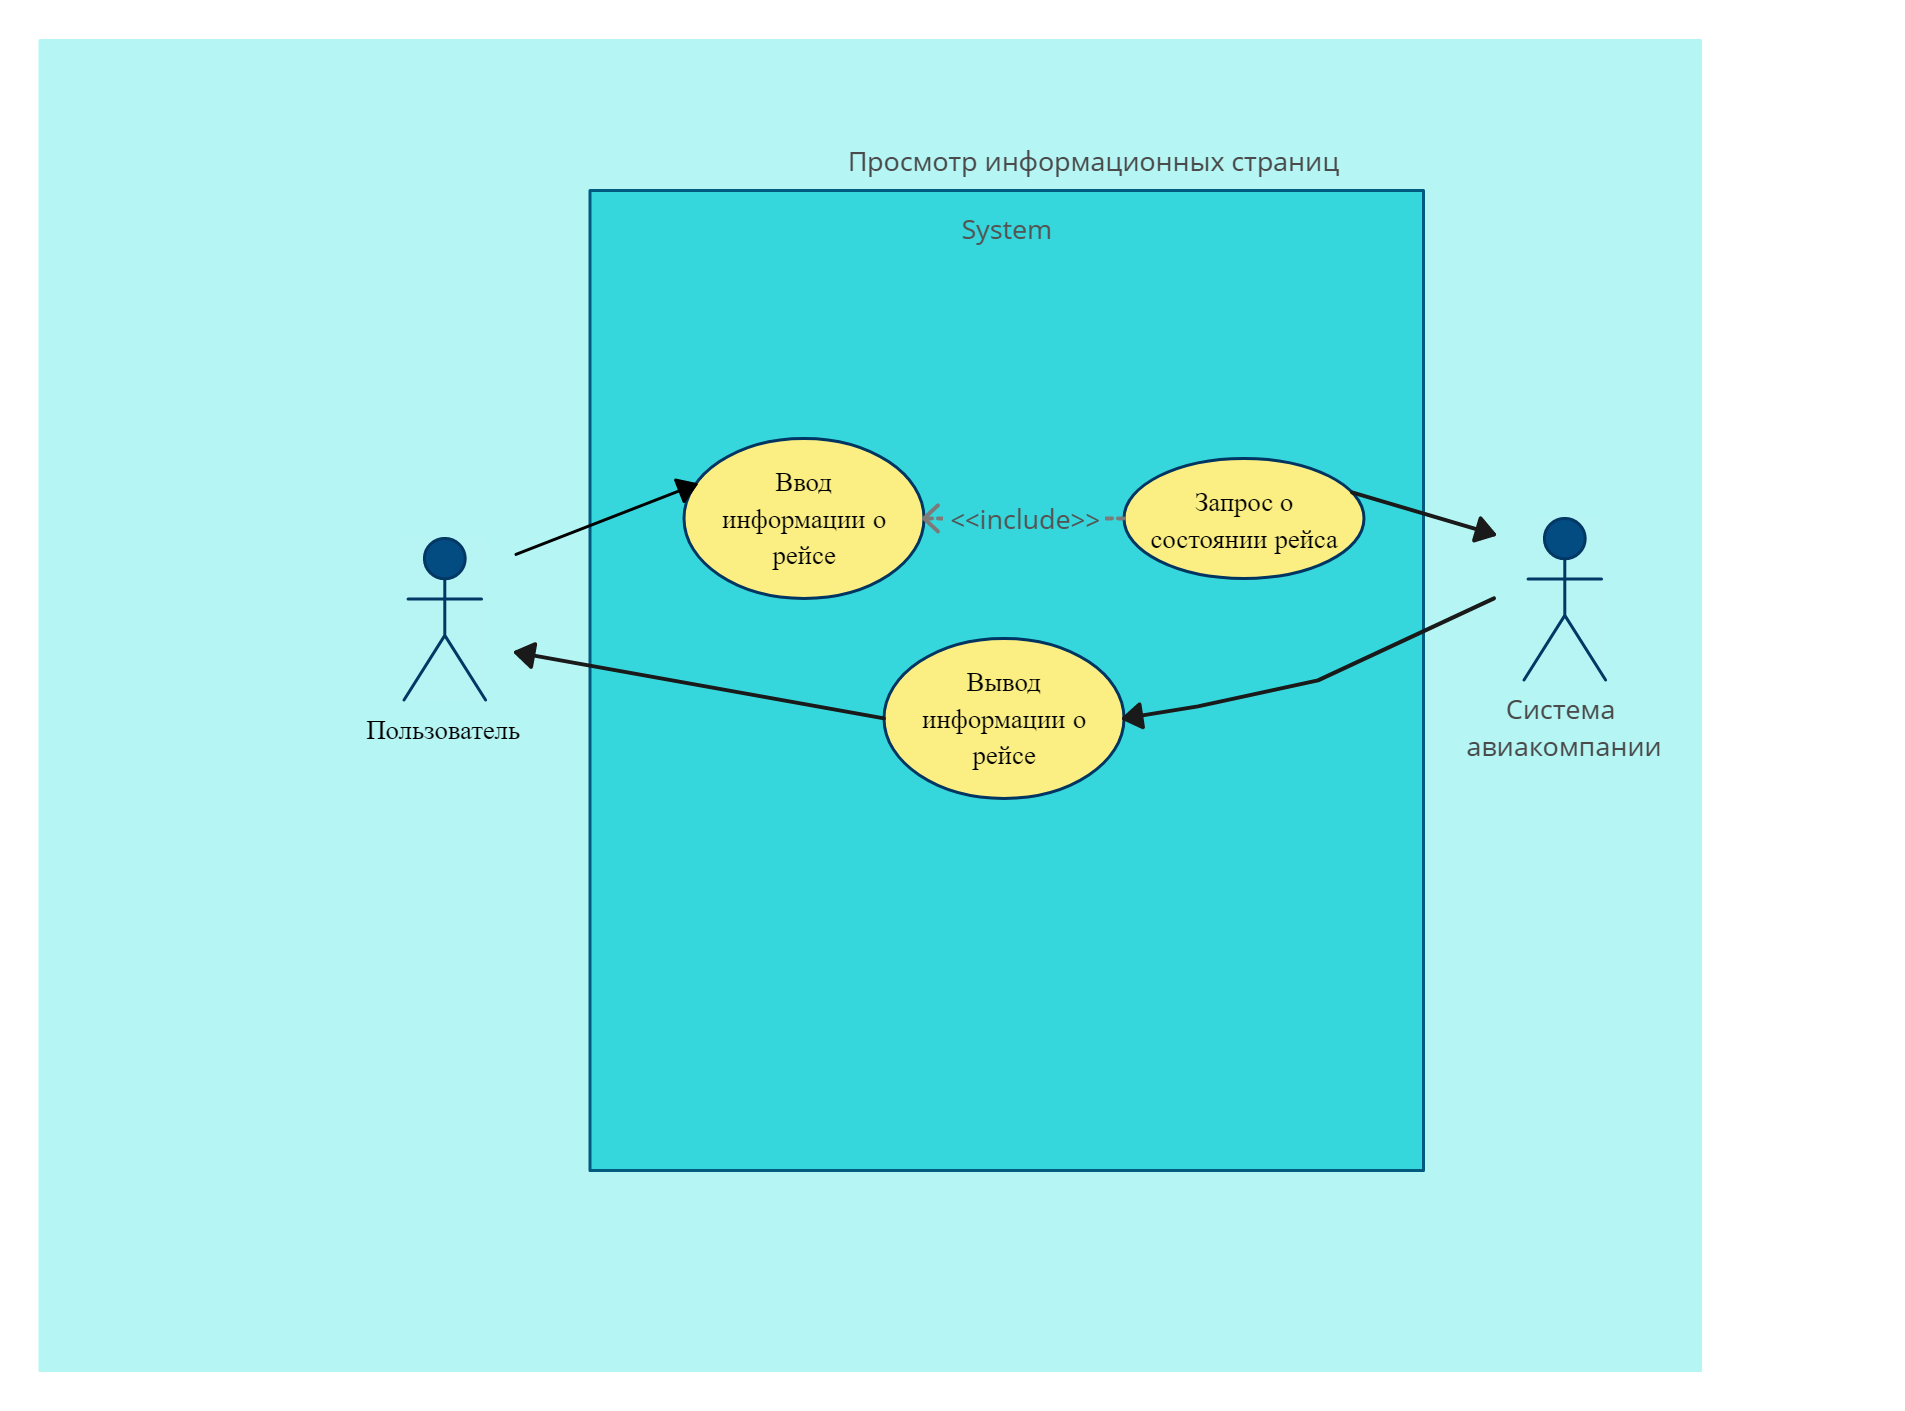
\includegraphics[width=16cm]{4-actions/Way_search.jpg}
      \centering
      \caption{Use-Case диаграмма: поиск рейса}
\end{figure}

\begin{figure}
      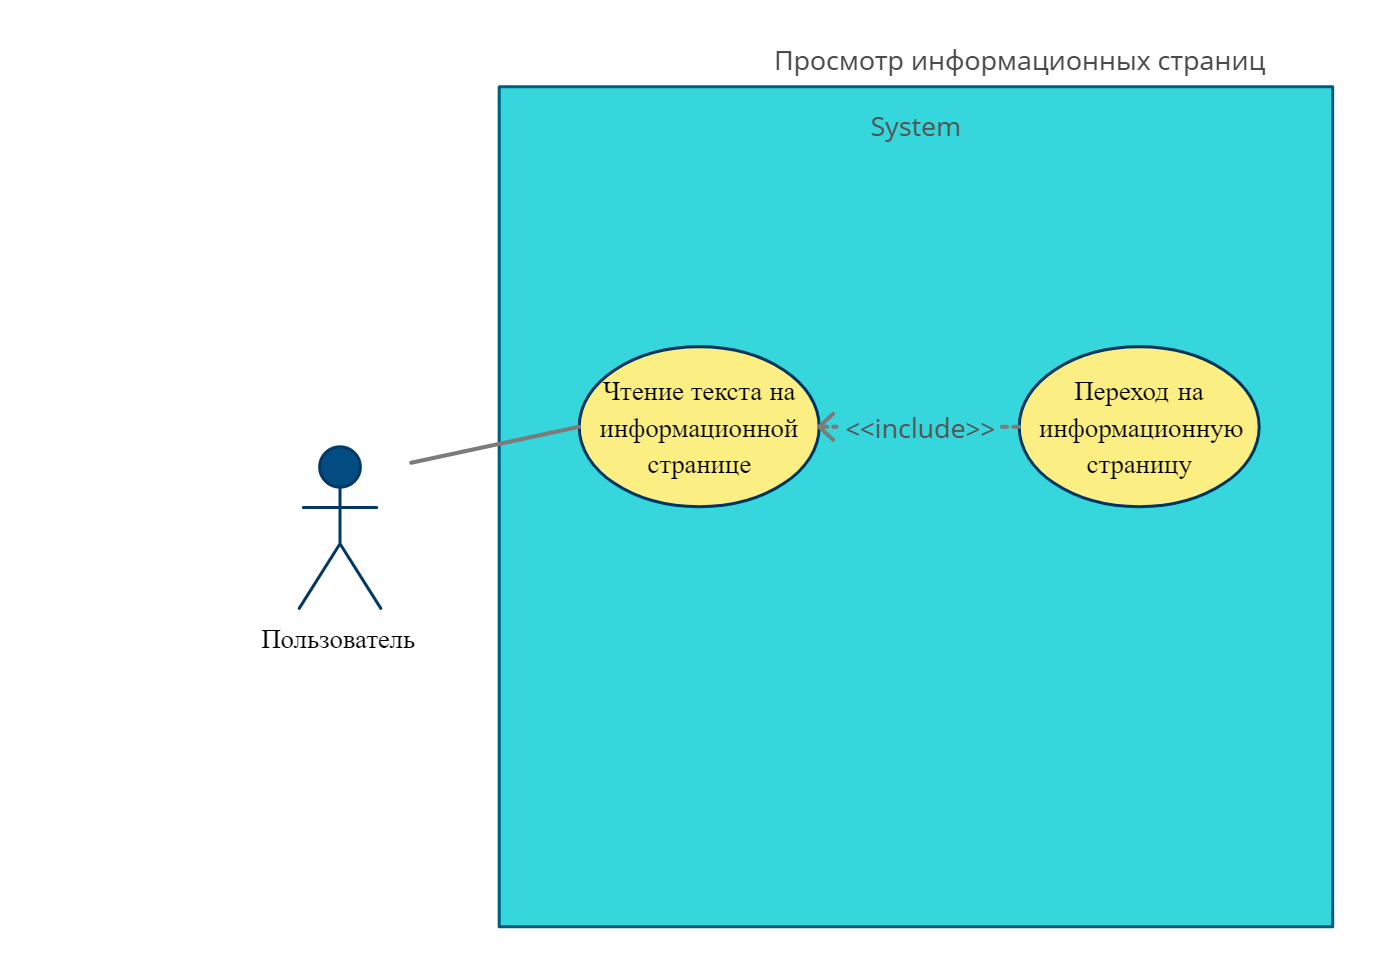
\includegraphics[width=16cm]{4-actions/Look_info_pages.jpg}
      \centering
      \caption{Use-Case диаграмма: просмотр пользователем информационных страниц}
\end{figure}

\begin{figure}
      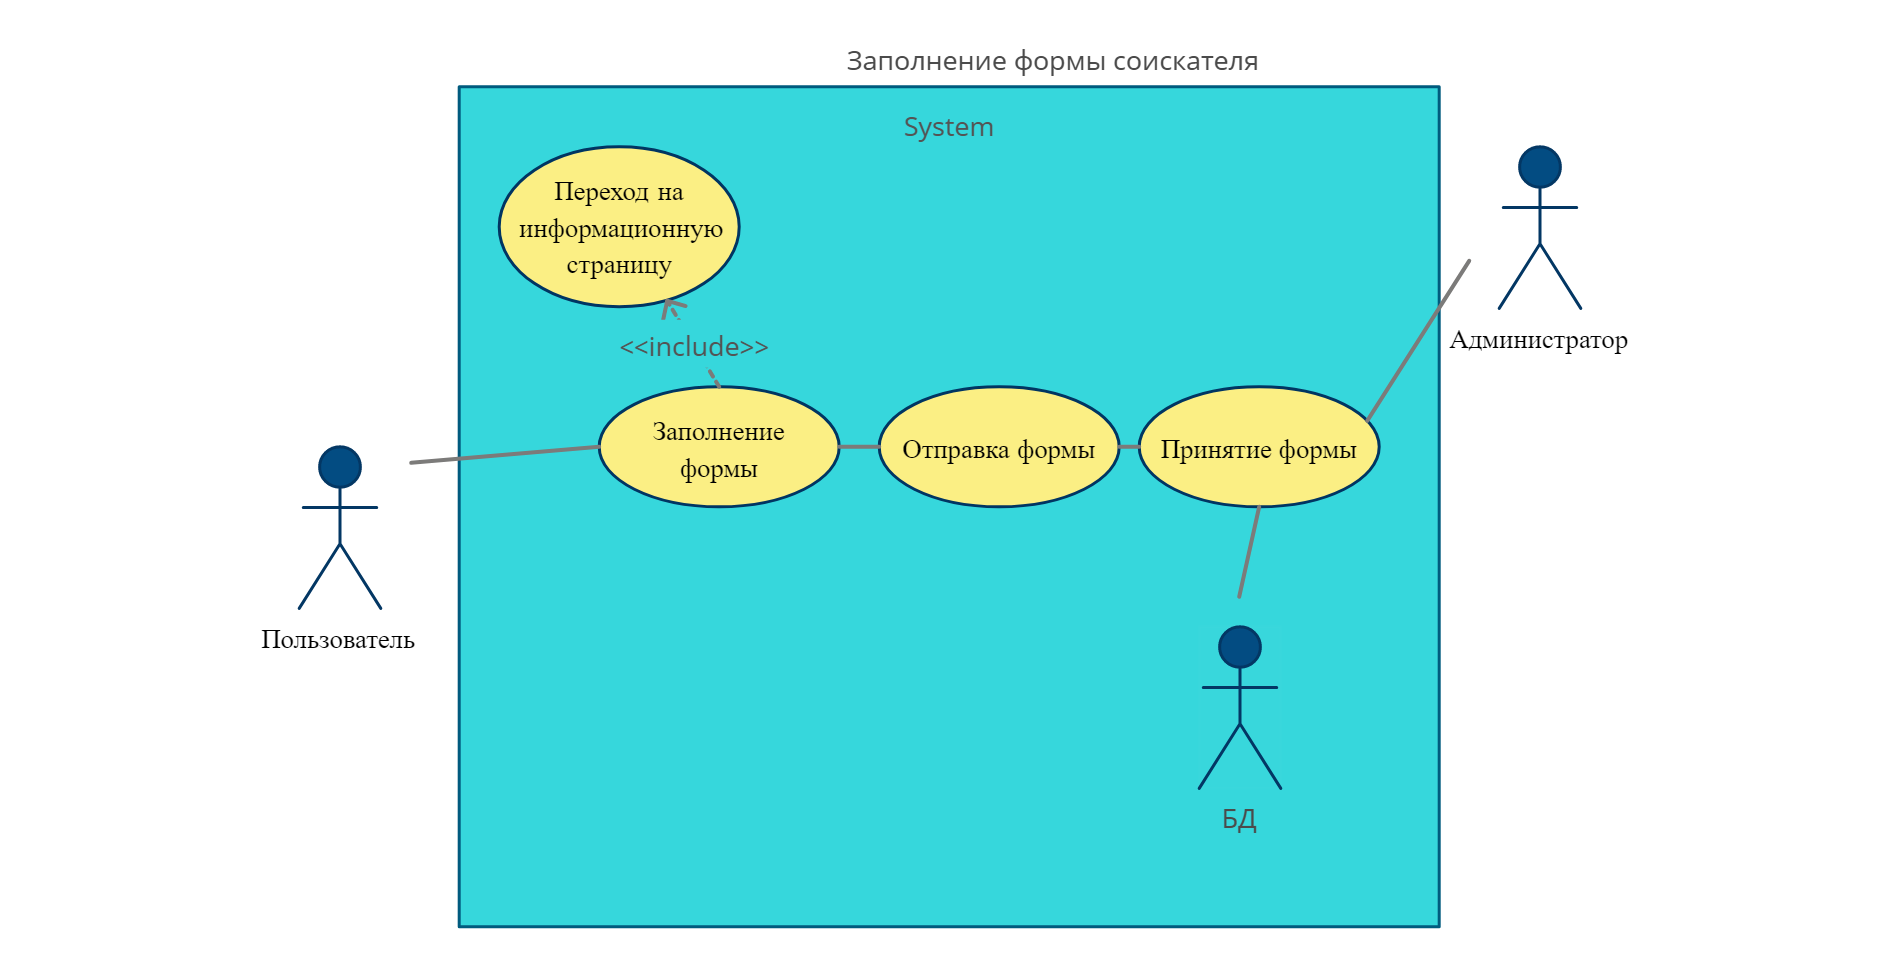
\includegraphics[width=16cm]{4-actions/Paper.jpg}
      \centering
      \caption{Use-Case диаграмма: заполнение формы}
\end{figure}

\begin{figure}
      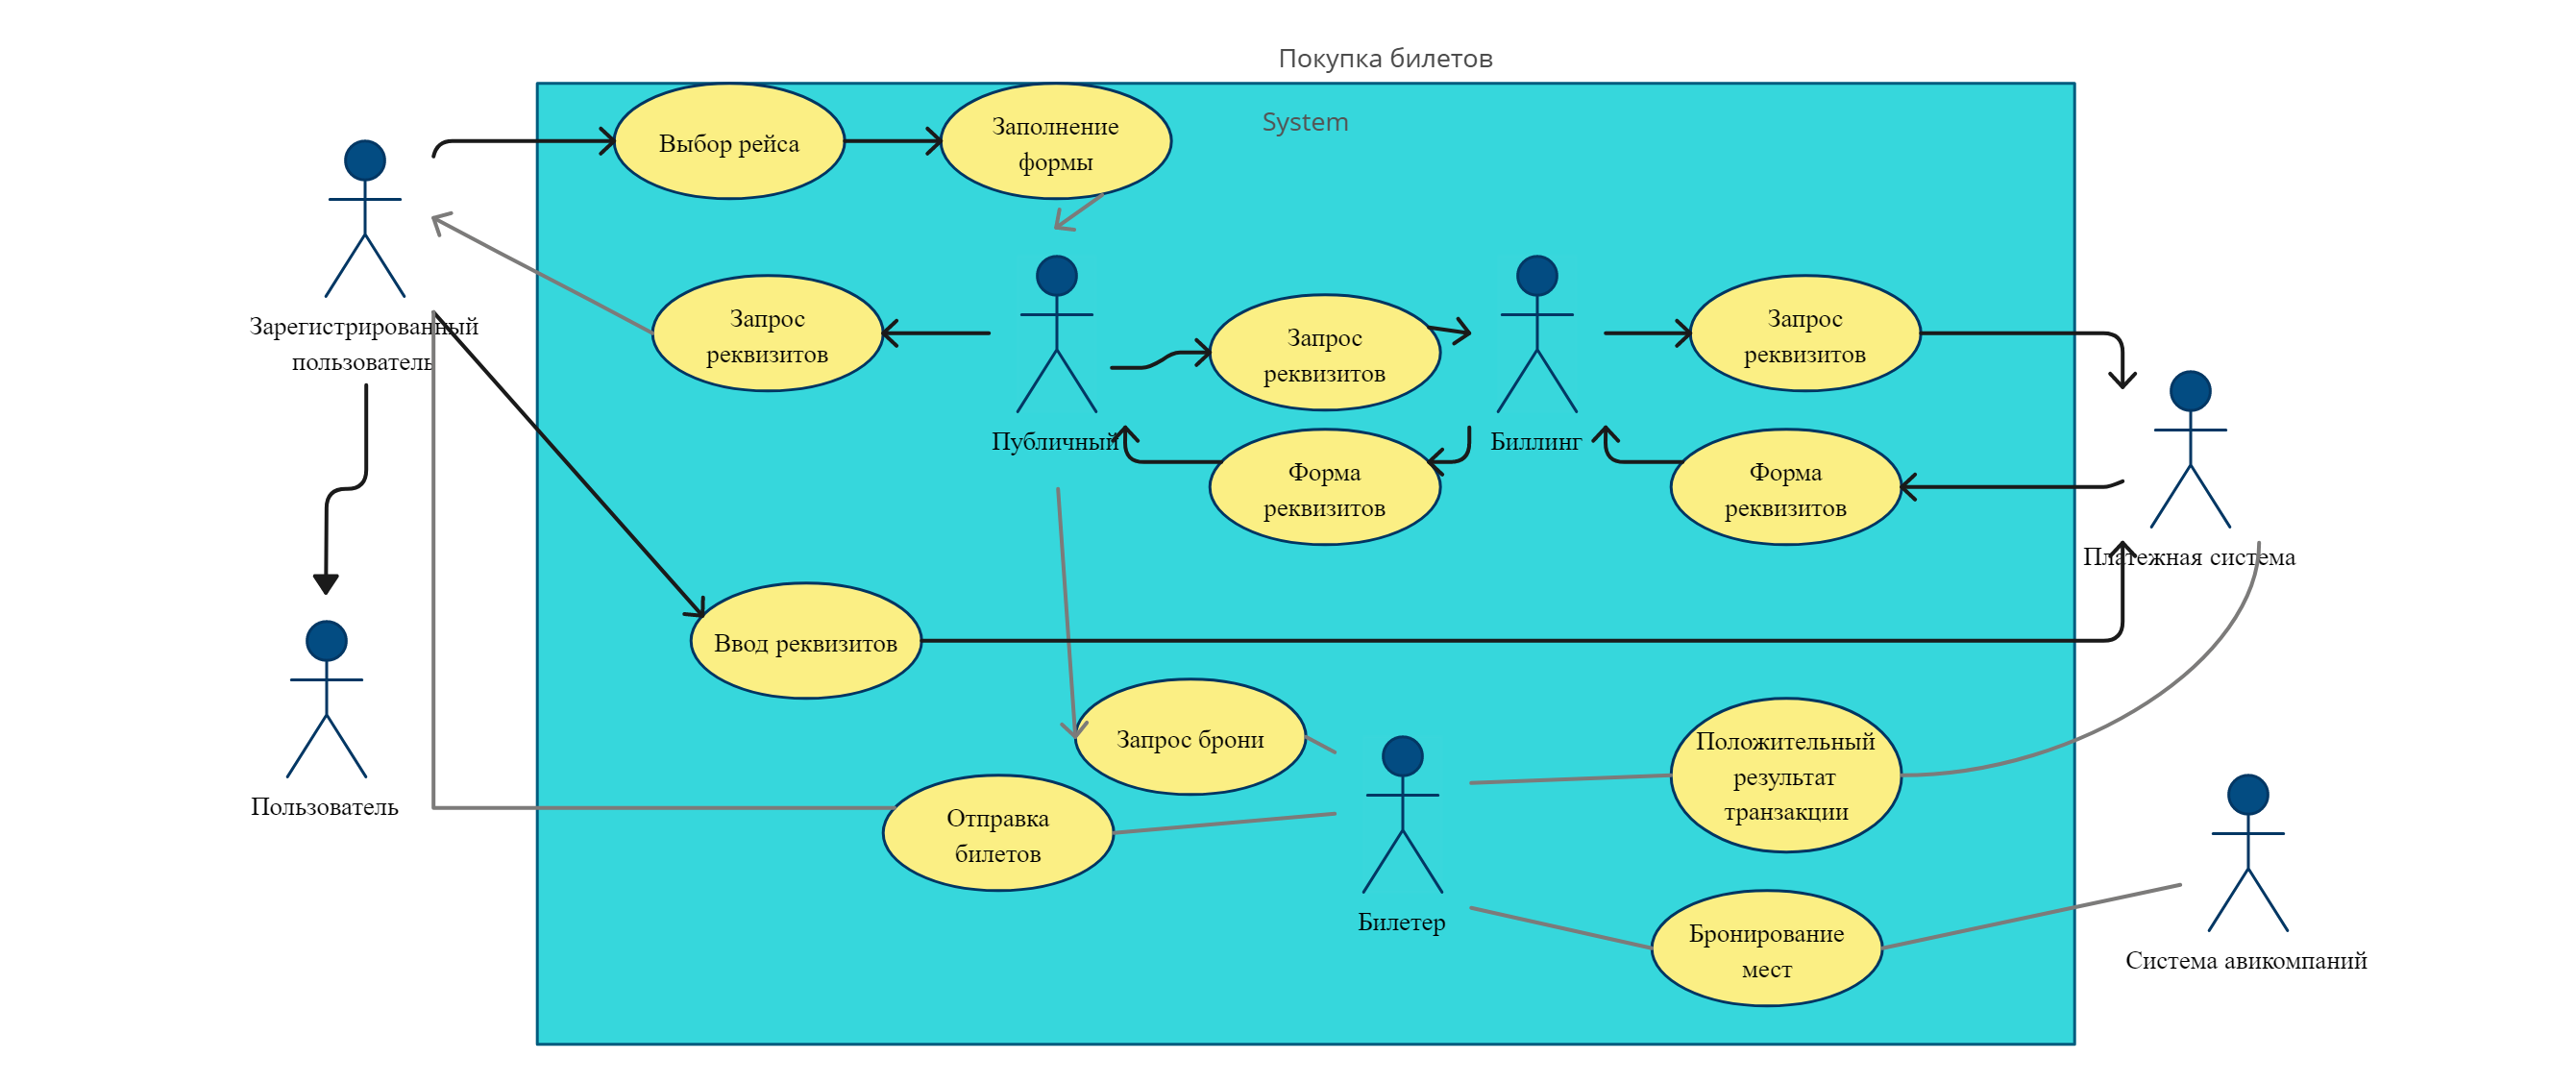
\includegraphics[width=16cm]{4-actions/Book_tickets.jpg}
      \centering
      \caption{Use-Case диаграмма: бронирование билета}
\end{figure}

\begin{figure}
      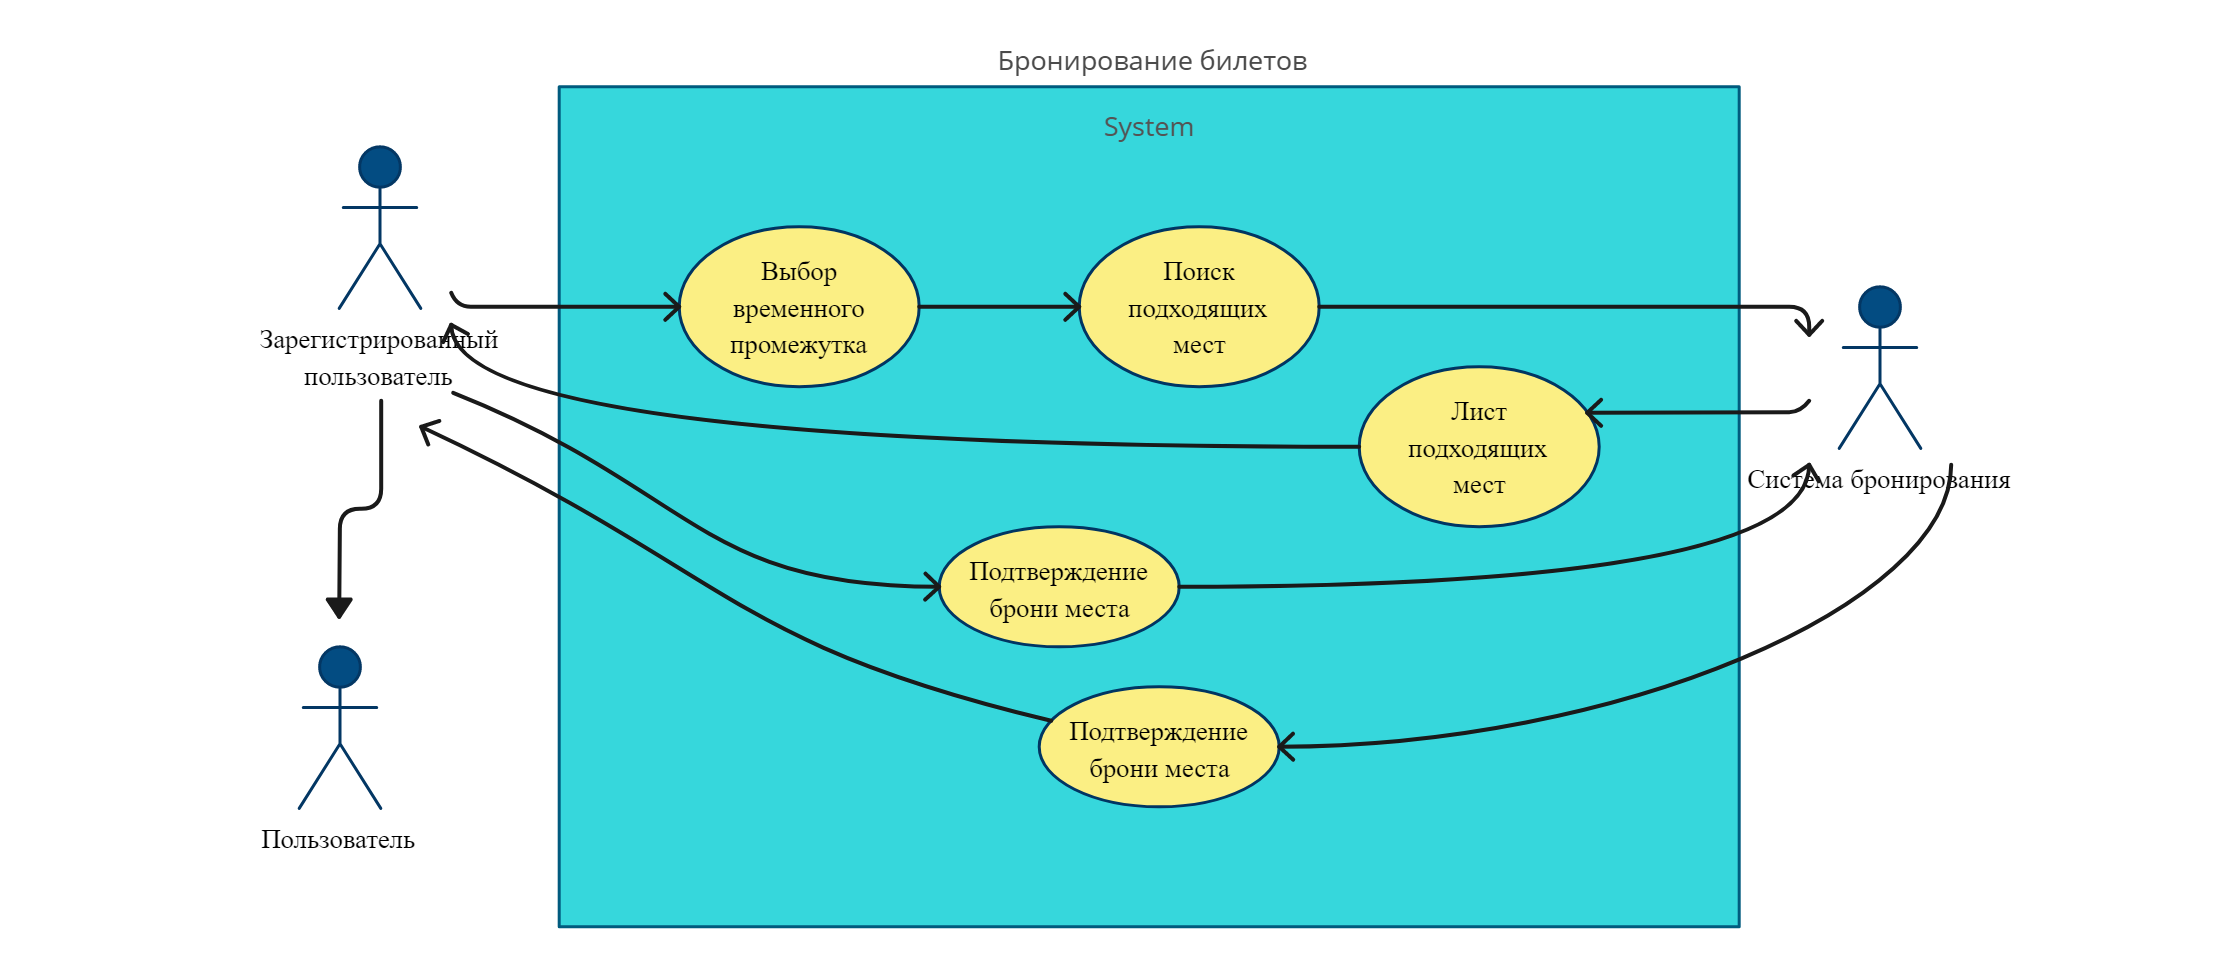
\includegraphics[width=16cm]{4-actions/Book_parking.jpg}
      \centering
      \caption{Use-Case диаграмма: бронирование паркинга}
\end{figure}

\begin{figure}
      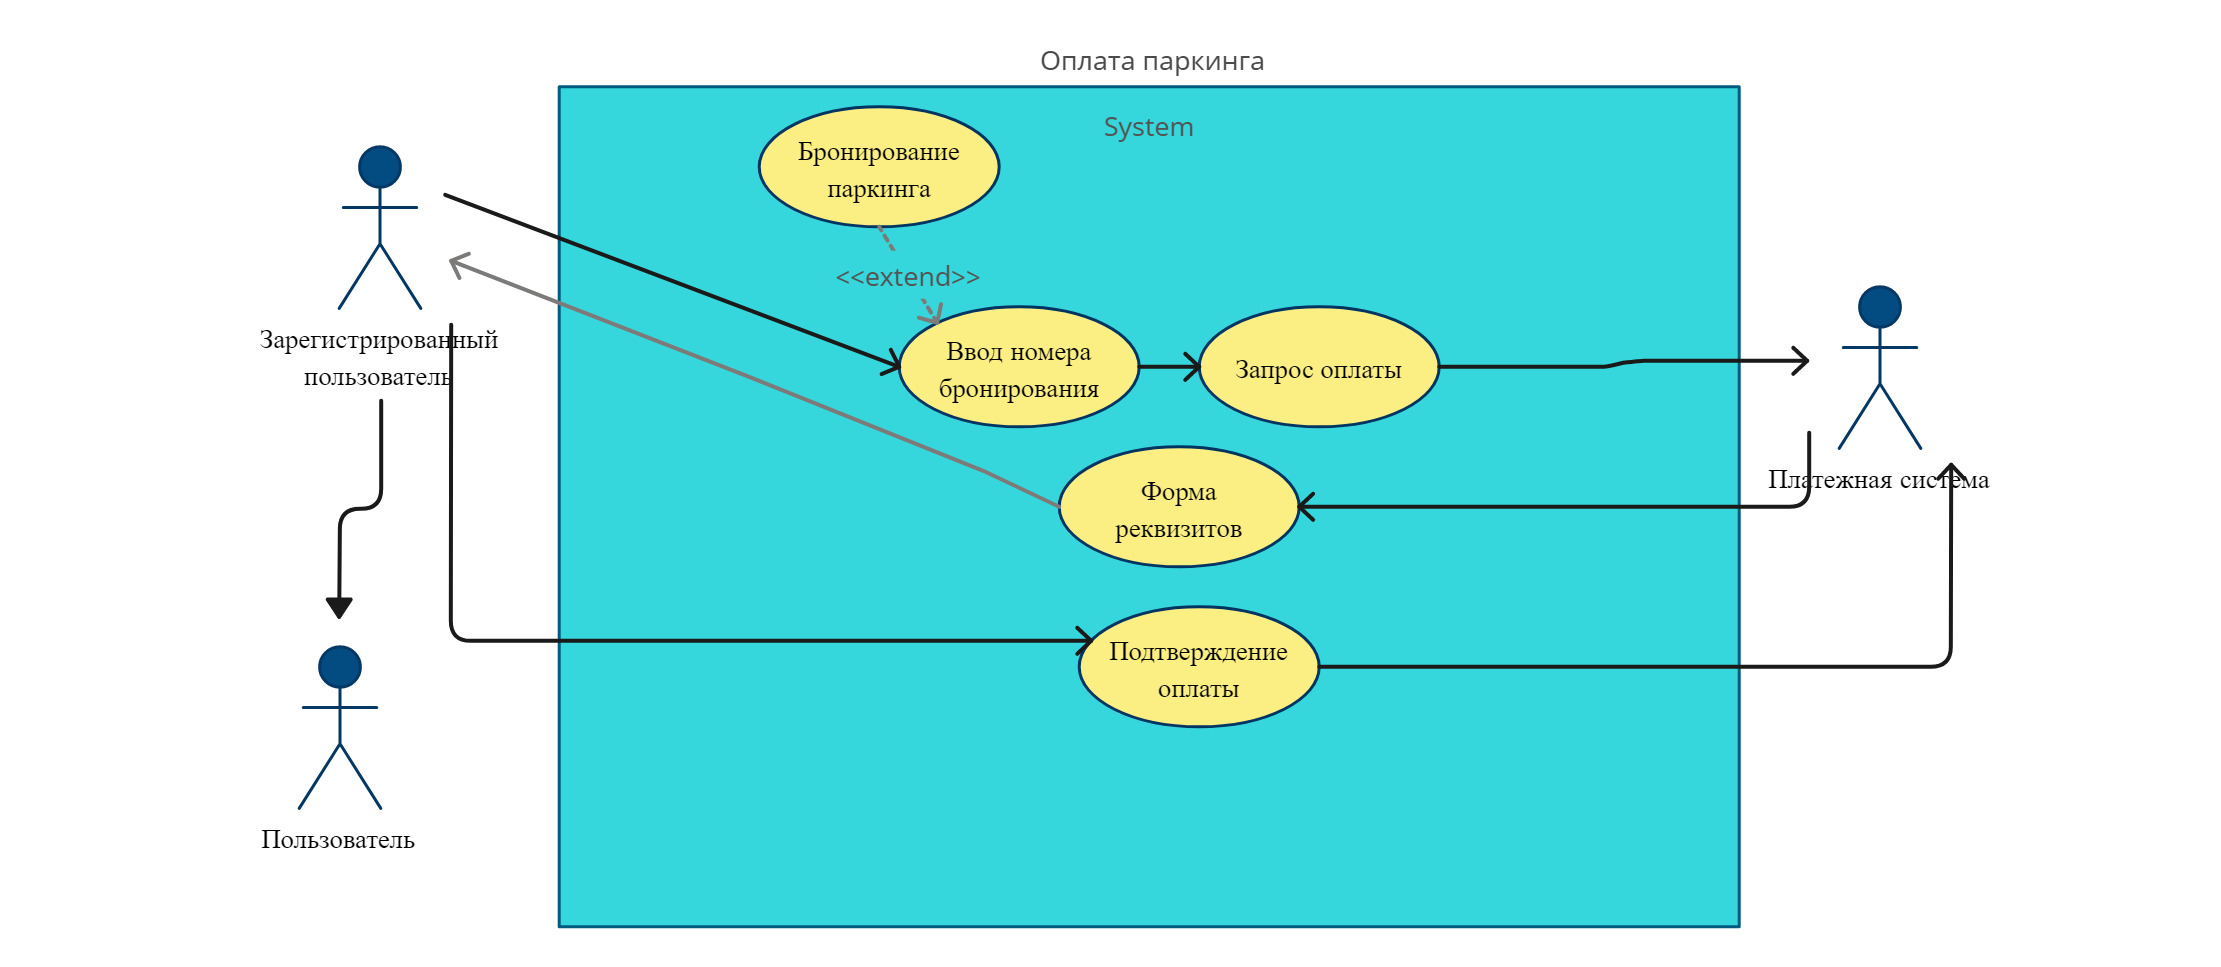
\includegraphics[width=16cm]{4-actions/Pay_parking.jpg}
      \centering
      \caption{Use-Case диаграмма: оплата паркинга}
\end{figure}

\begin{figure}
      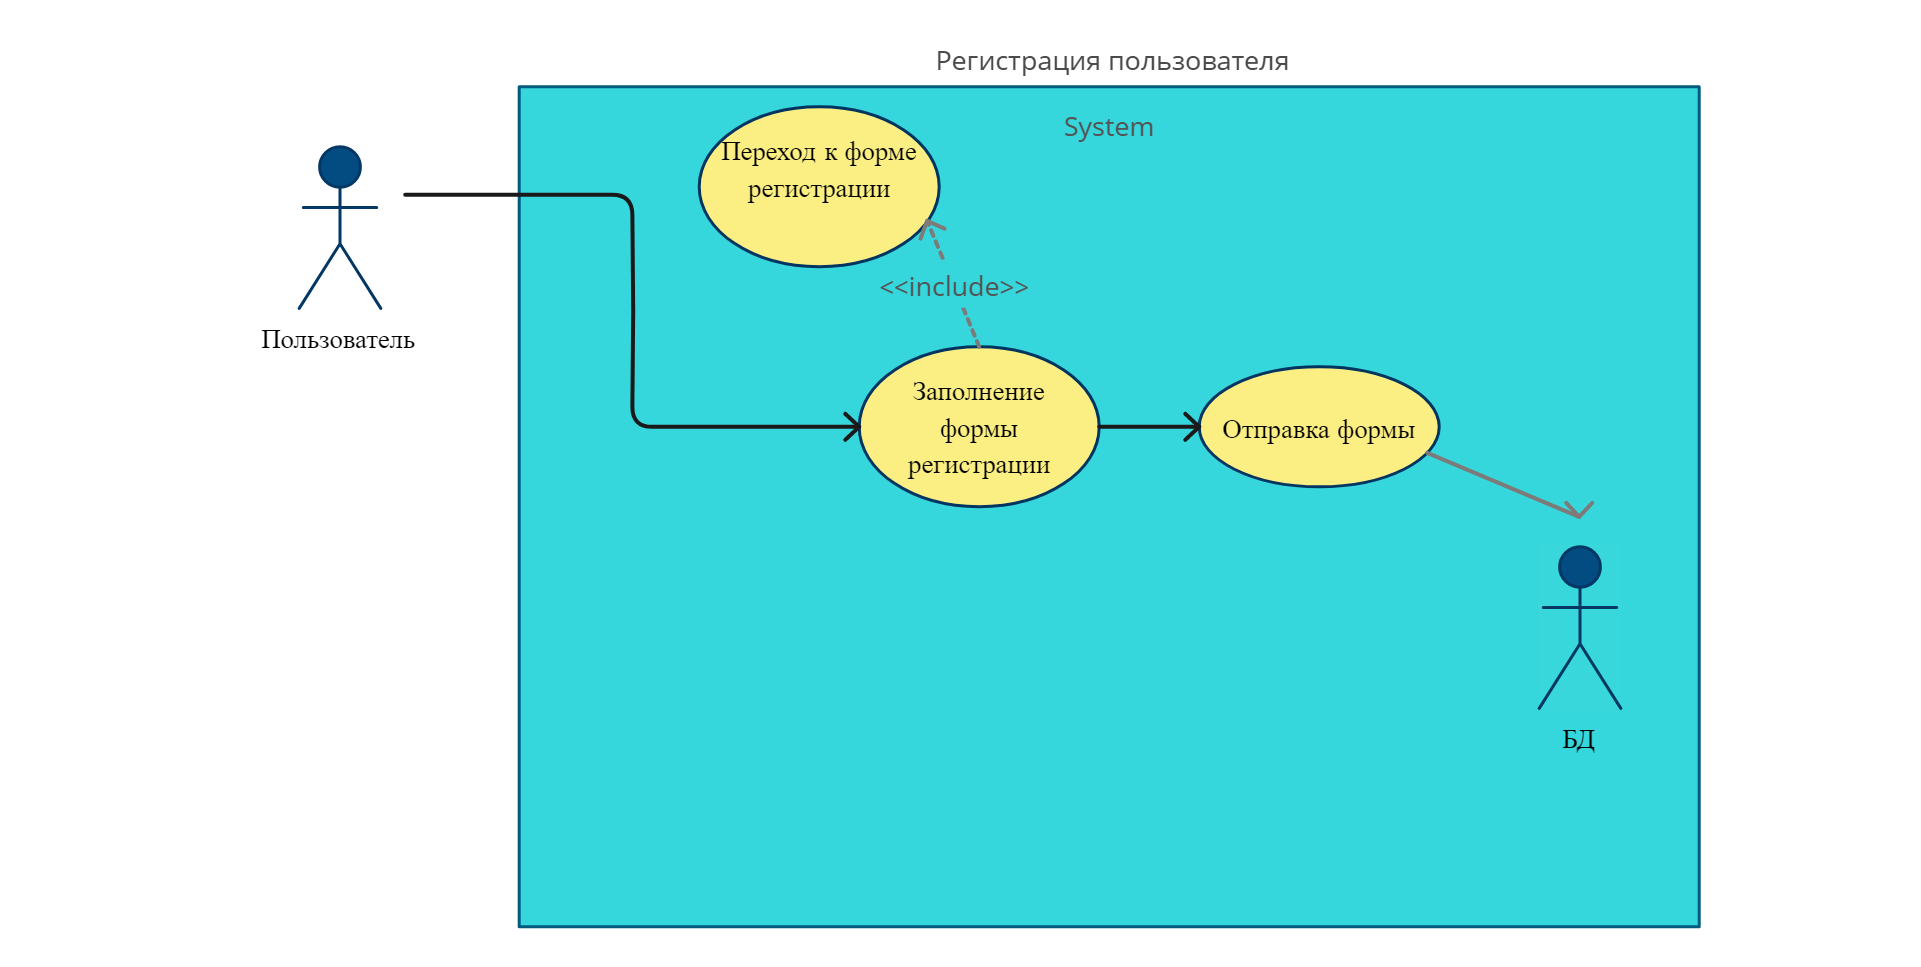
\includegraphics[width=16cm]{4-actions/Registration.jpg}
      \centering
      \caption{Use-Case диаграмма: регистрация на сайте}
\end{figure}

\begin{figure}
      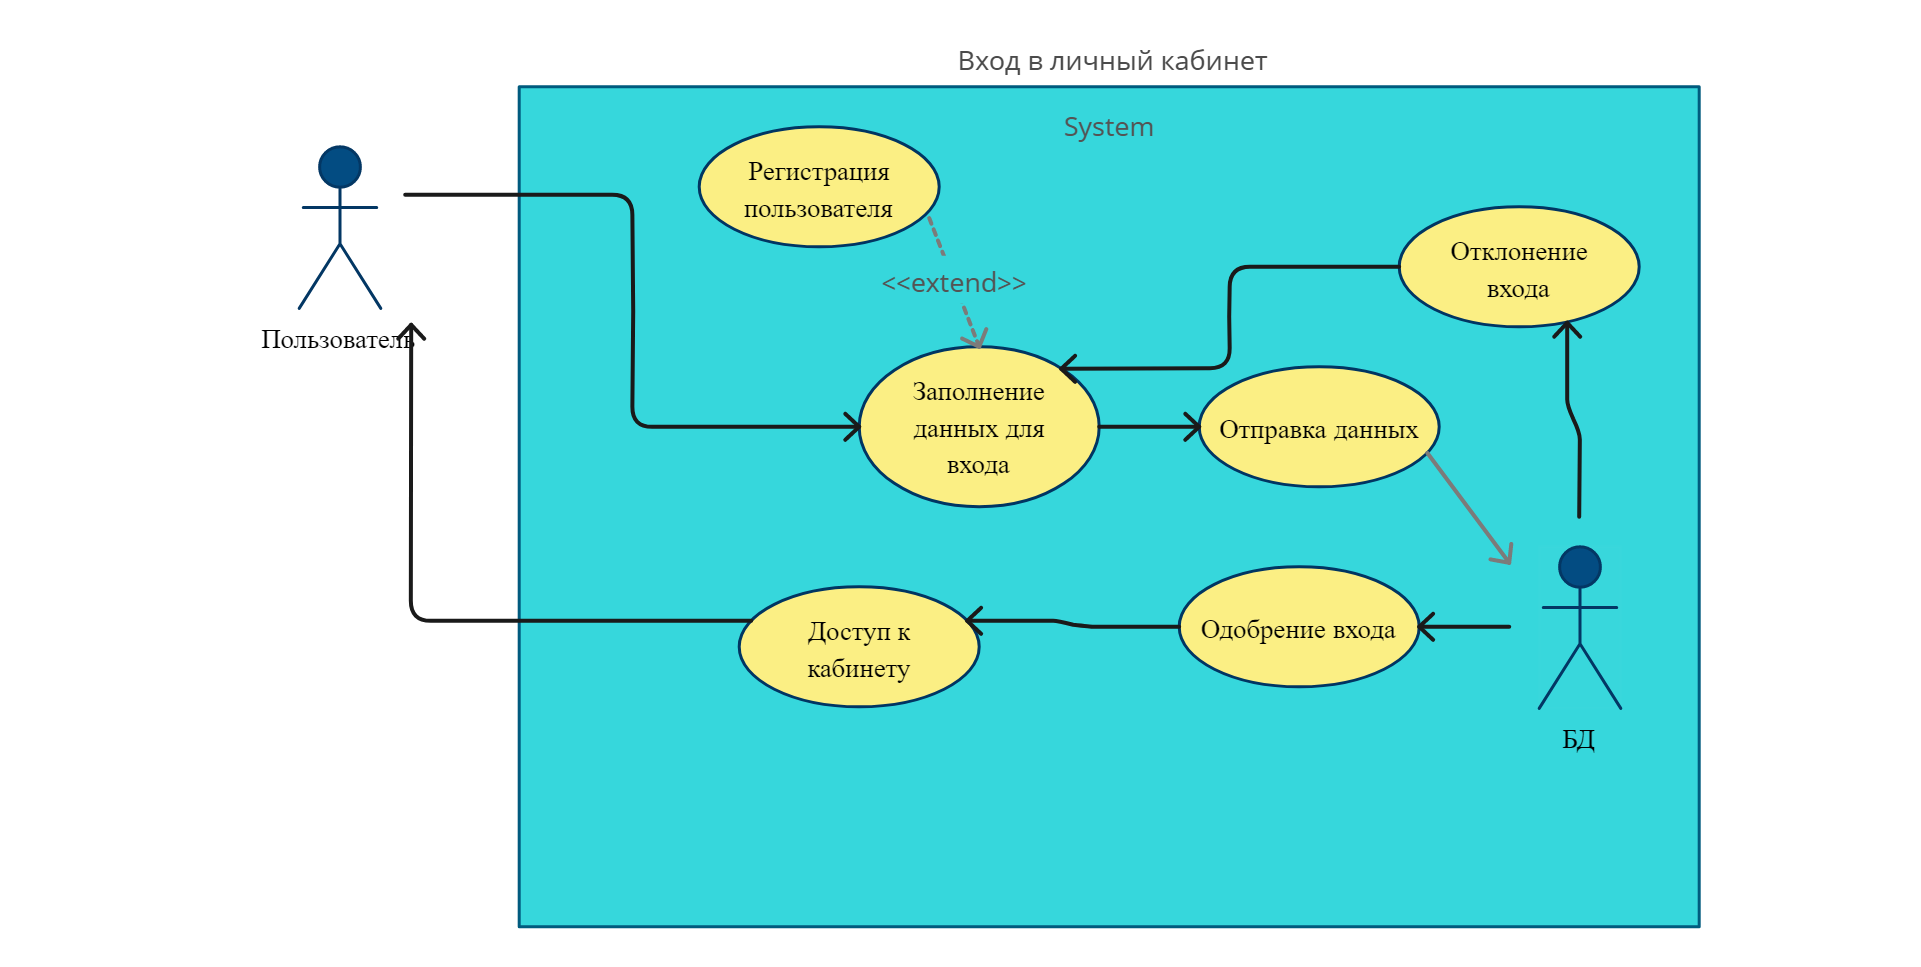
\includegraphics[width=16cm]{4-actions/Enter.jpg}
      \centering
      \caption{Use-Case диаграмма: вход в личный кабинет}
\end{figure}

\begin{figure}
      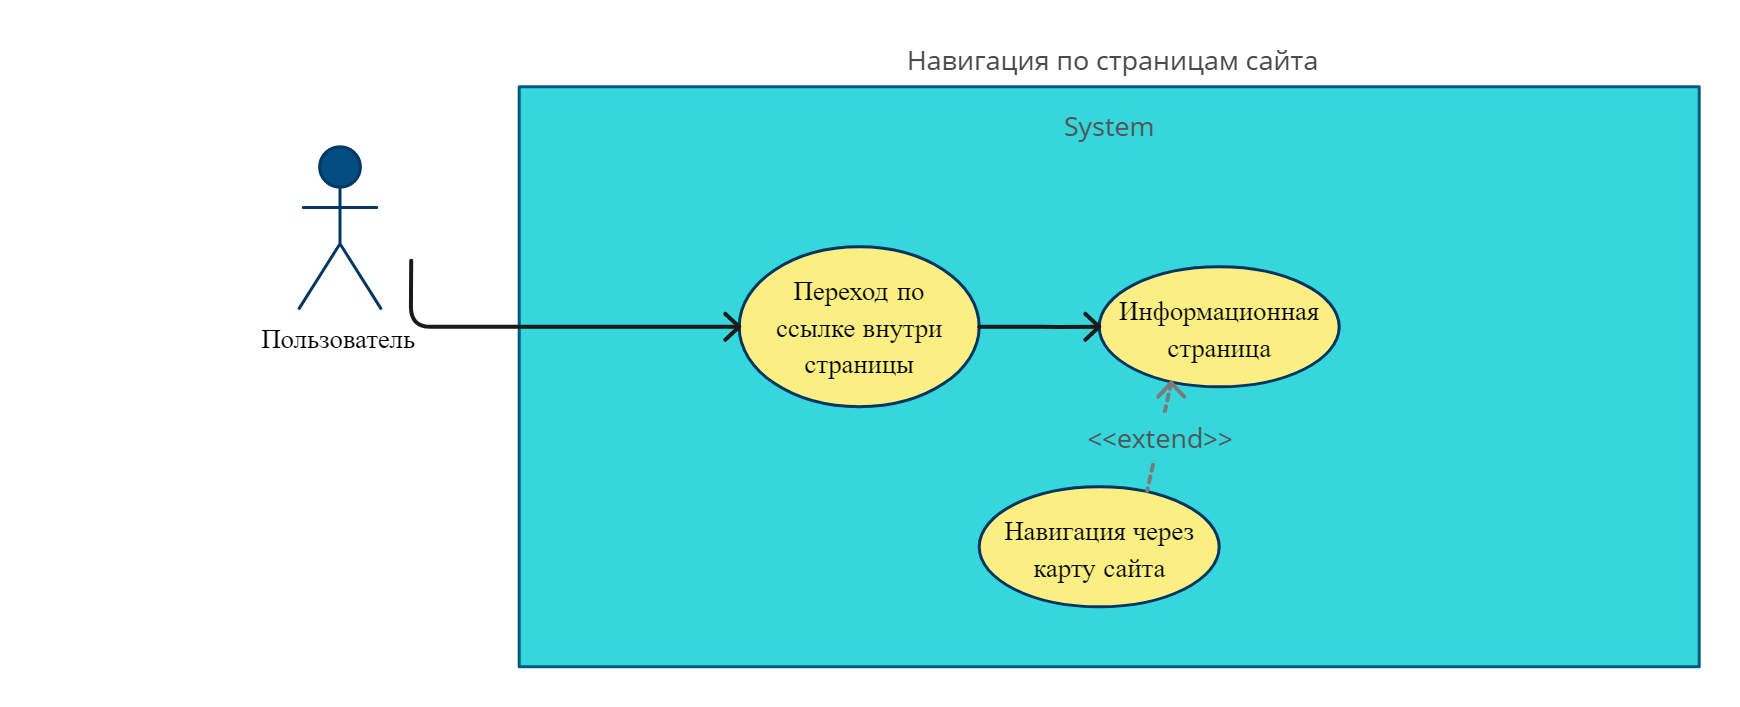
\includegraphics[width=16cm]{4-actions/Navigation.jpg}
      \centering
      \caption{Use-Case диаграмма: навигация между страницами сайта}
\end{figure}

\begin{figure}
      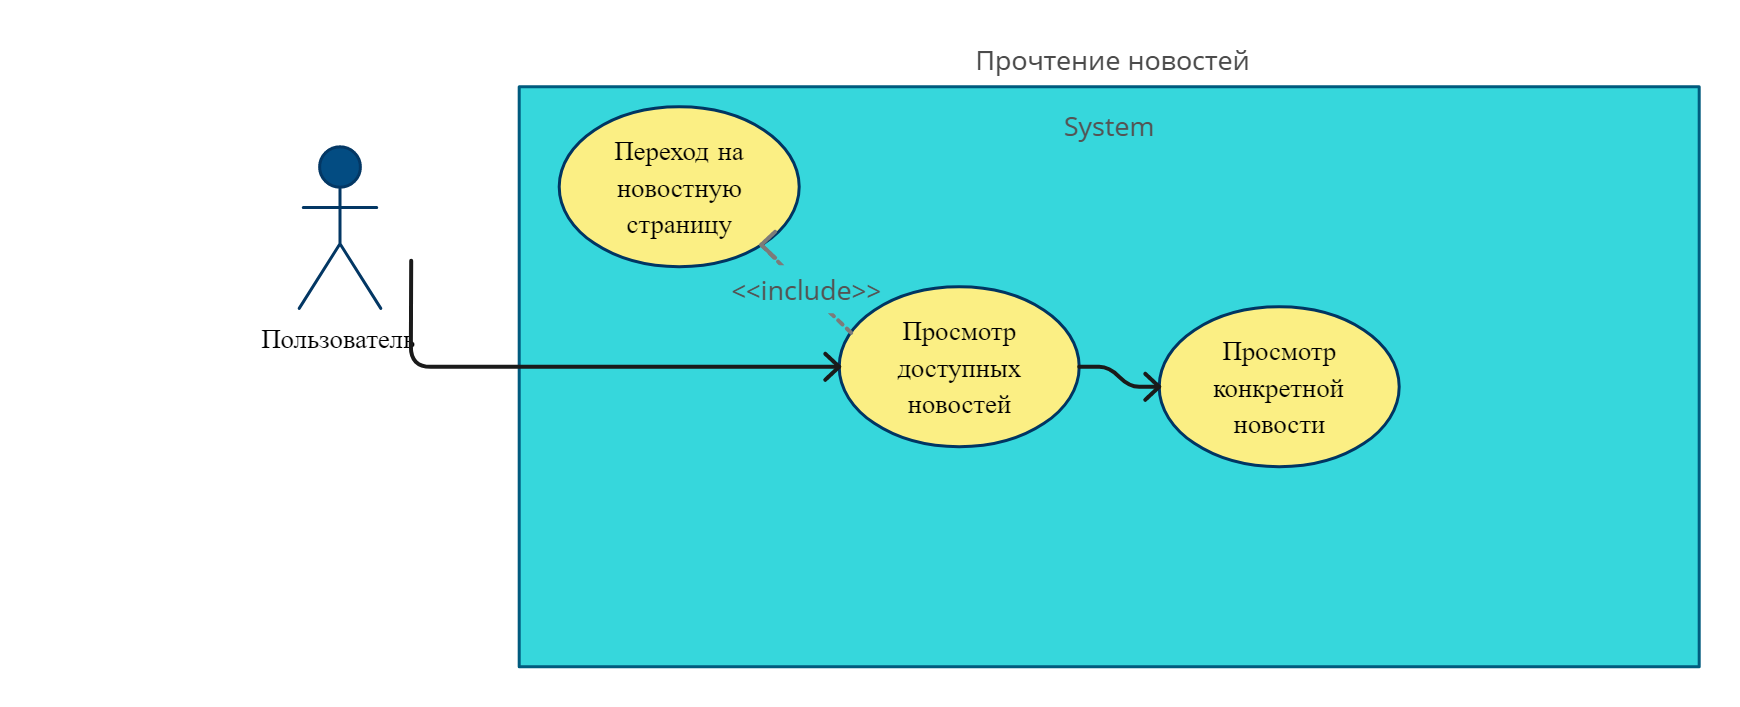
\includegraphics[width=16cm]{4-actions/News.jpg}
      \centering
      \caption{Use-Case диаграмма: просмотр новостей}
\end{figure}

\begin{figure}
      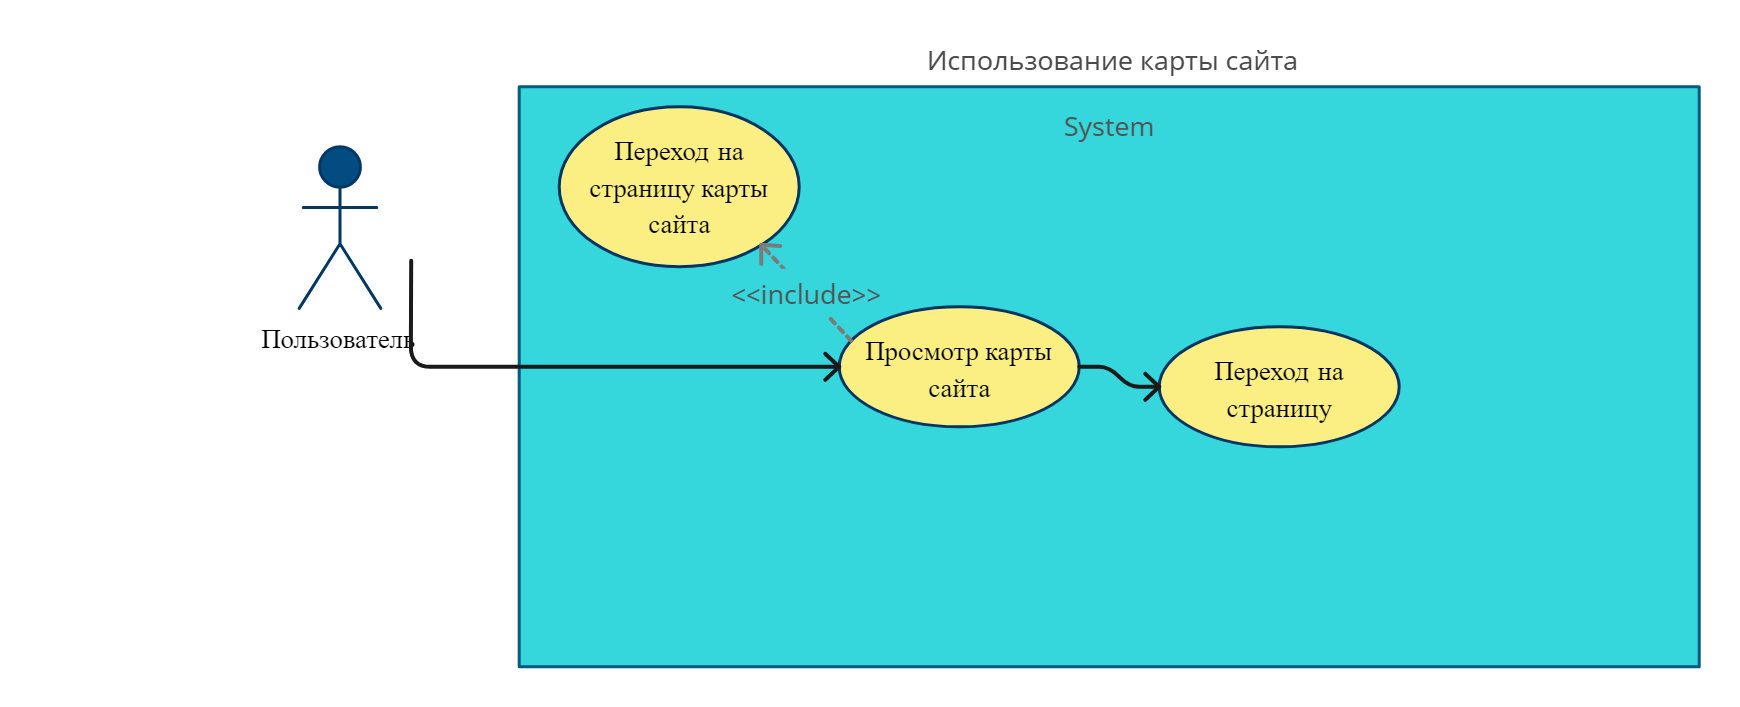
\includegraphics[width=16cm]{4-actions/App_map.jpg}
      \centering
      \caption{Use-Case диаграмма: использование карты сайта}
\end{figure}

\begin{figure}
      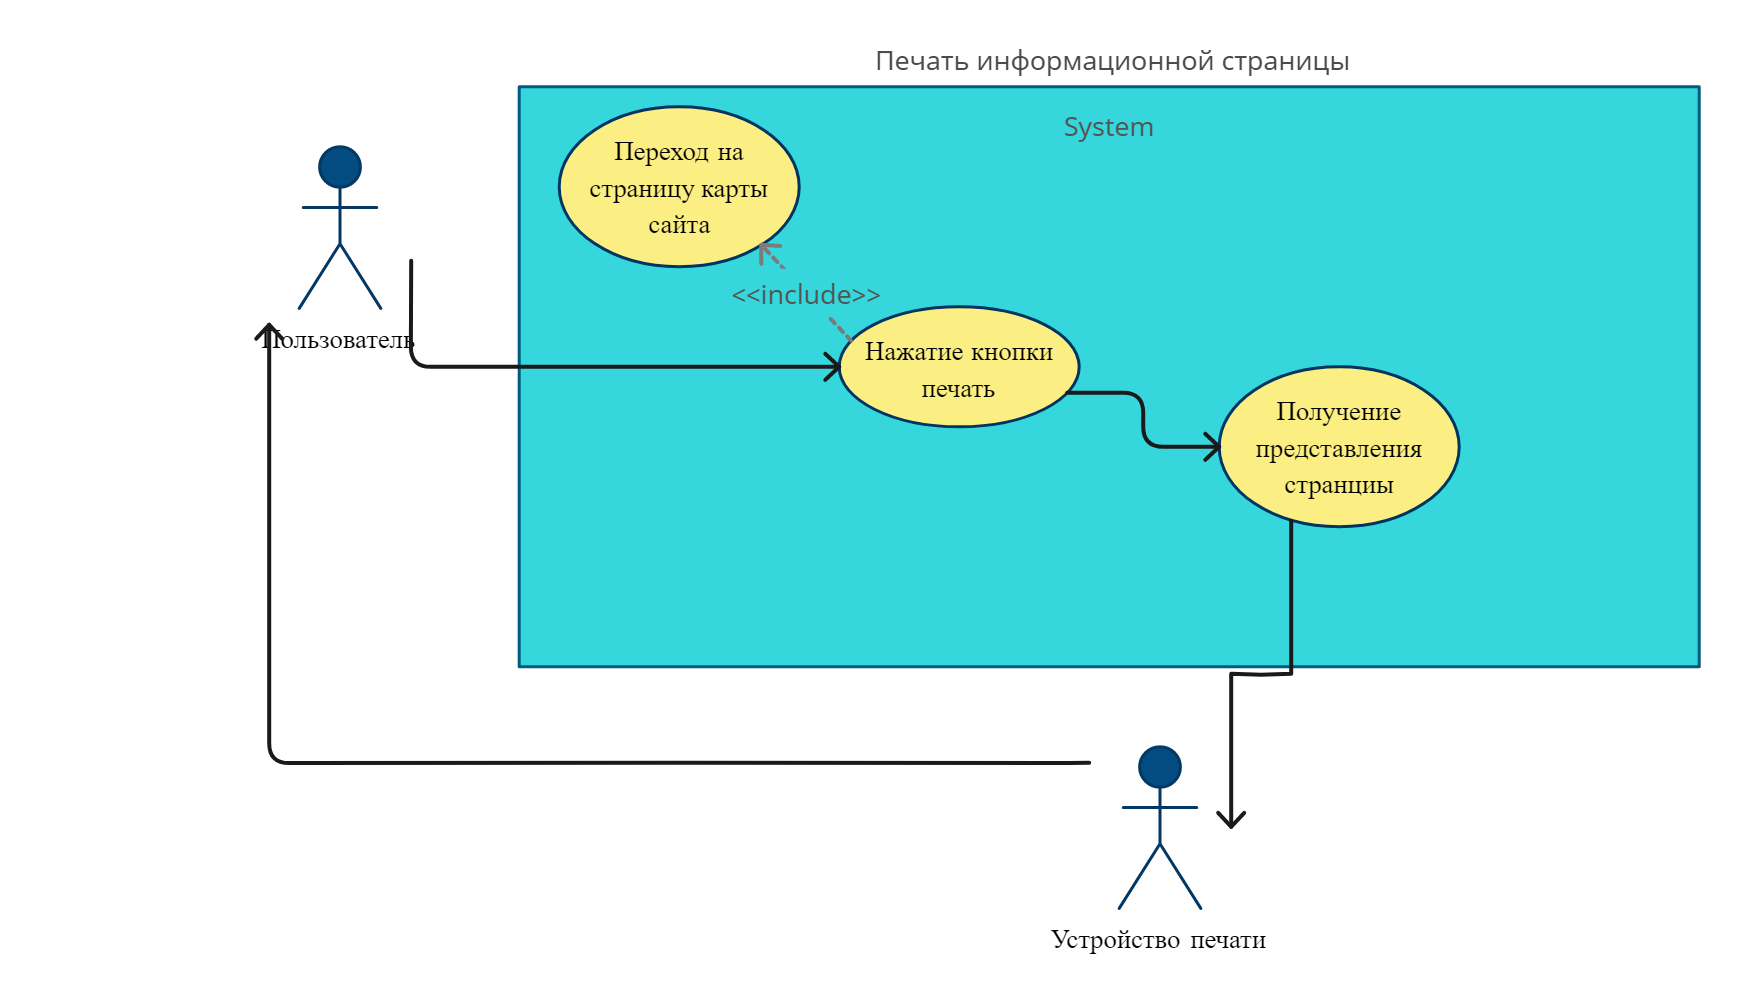
\includegraphics[width=16cm]{4-actions/Print.jpg}
      \centering
      \caption{Use-Case диаграмма: печать информационных страниц}
\end{figure}

\begin{figure}
      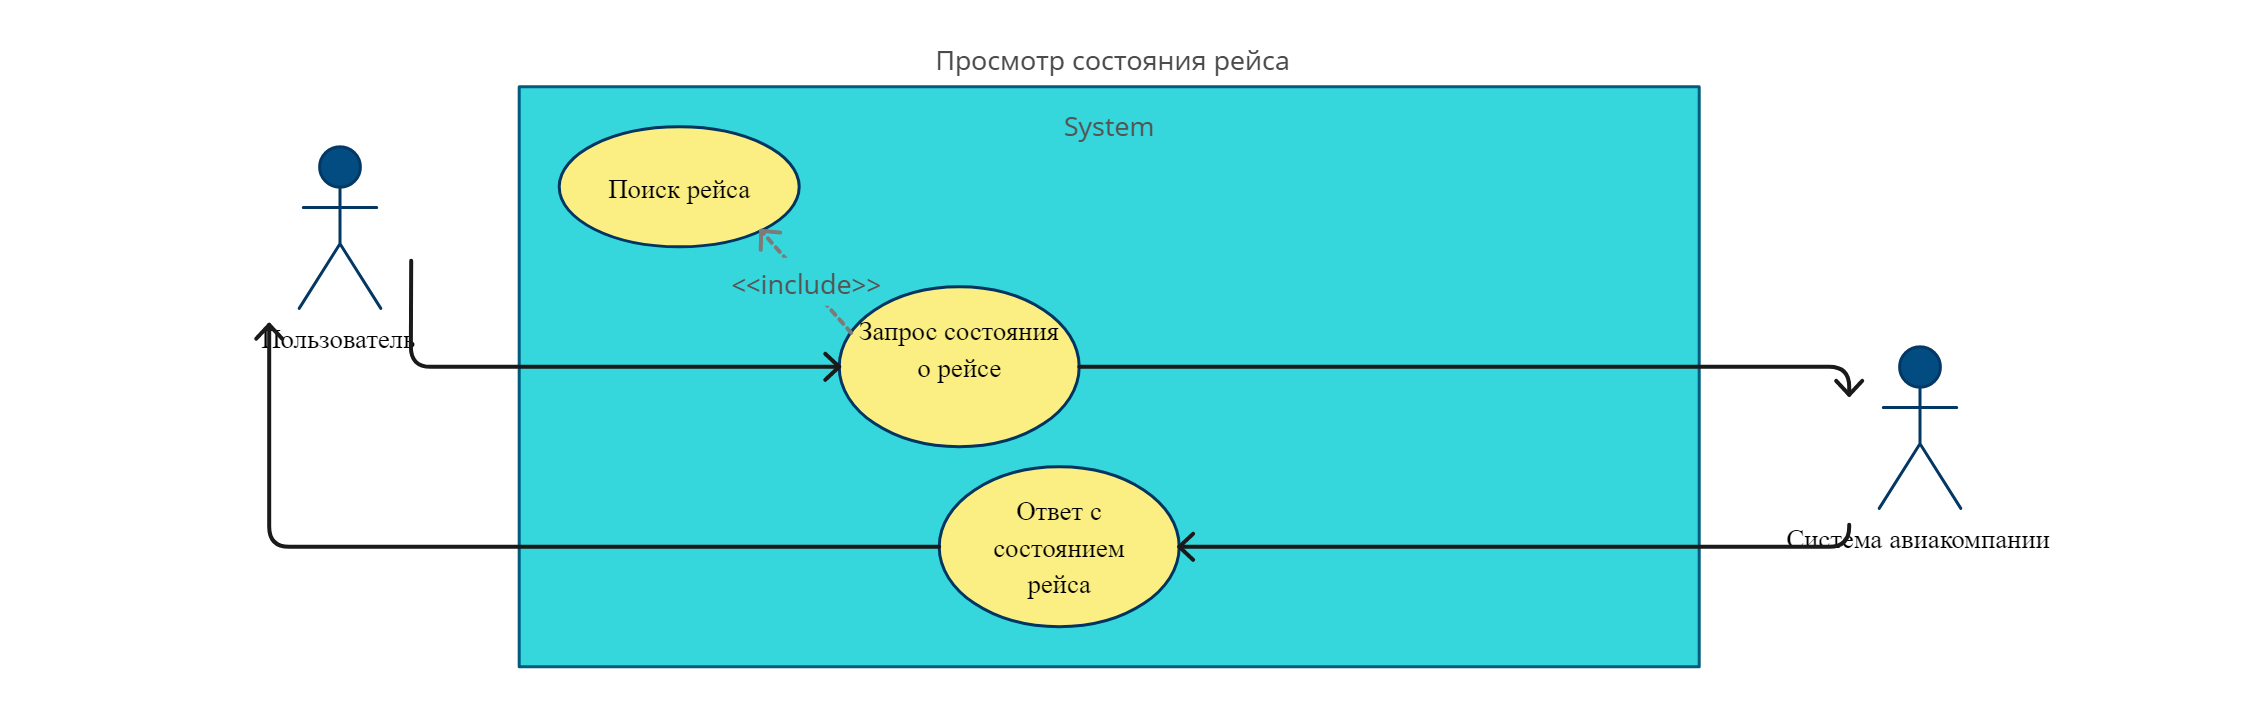
\includegraphics[width=16cm]{4-actions/Flight-state.jpg}
      \centering
      \caption{Use-Case диаграмма: просмотр состояния рейса}
\end{figure}

\begin{figure}
      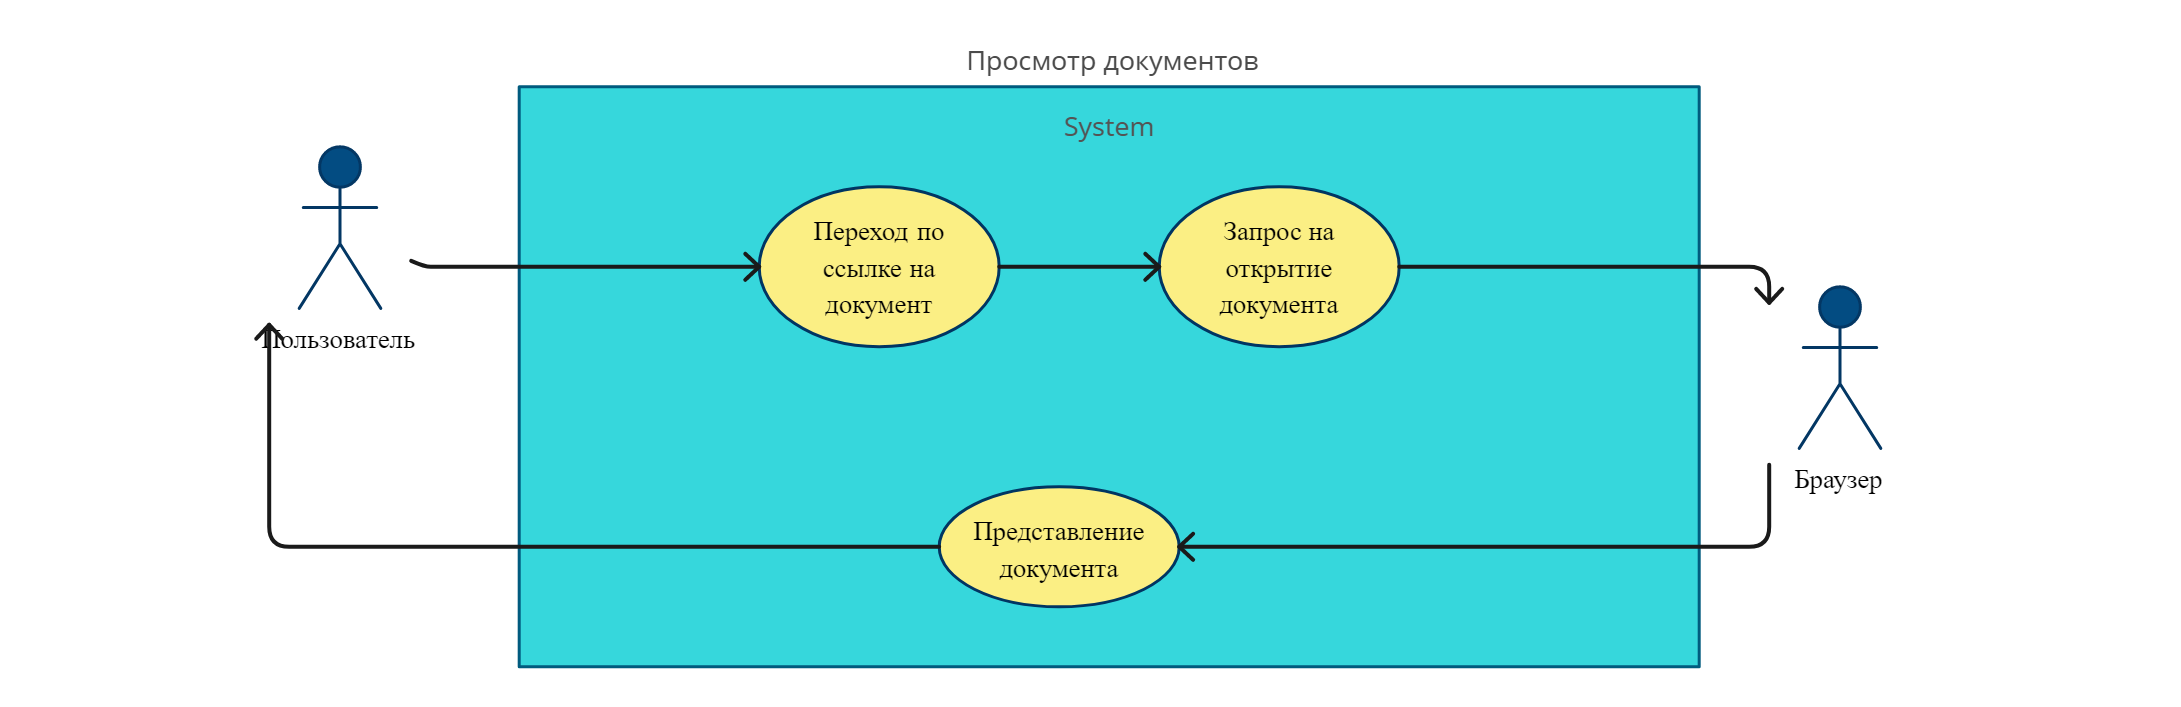
\includegraphics[width=16cm]{4-actions/Documents.jpg}
      \centering
      \caption{Use-Case диаграмма: просмотр вложенных документов}
\end{figure}

\begin{figure}
      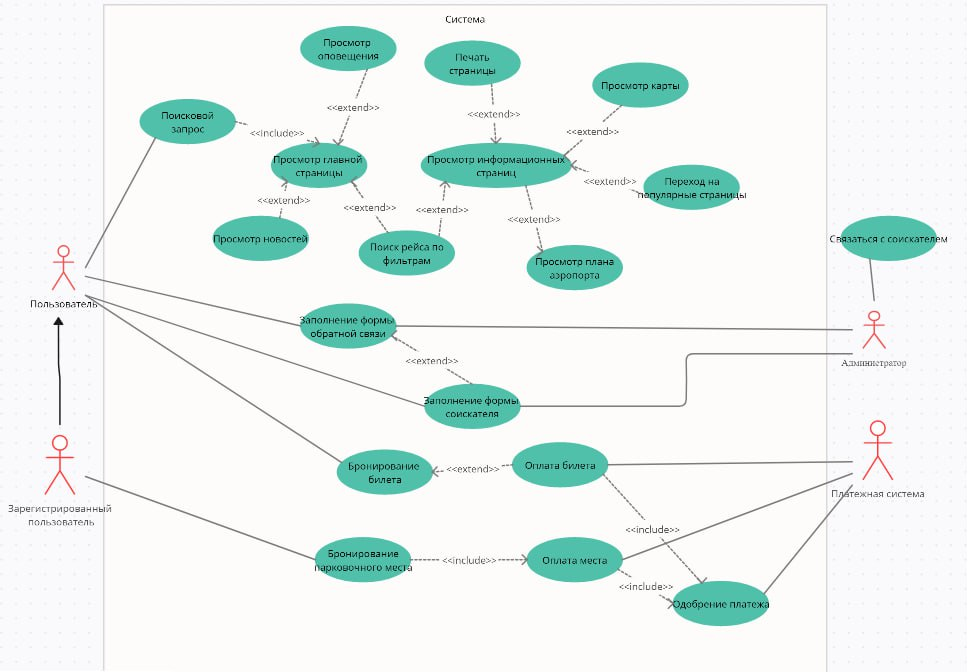
\includegraphics[width=16cm]{4-actions/use-case.jpg}
      \centering
      \caption{Use-Case диаграмма: вся система}
\end{figure}


\newpage
\section{Use-case диаграмма}

\subsection{Use-case диаграмма}
\begin{figure}[h]
  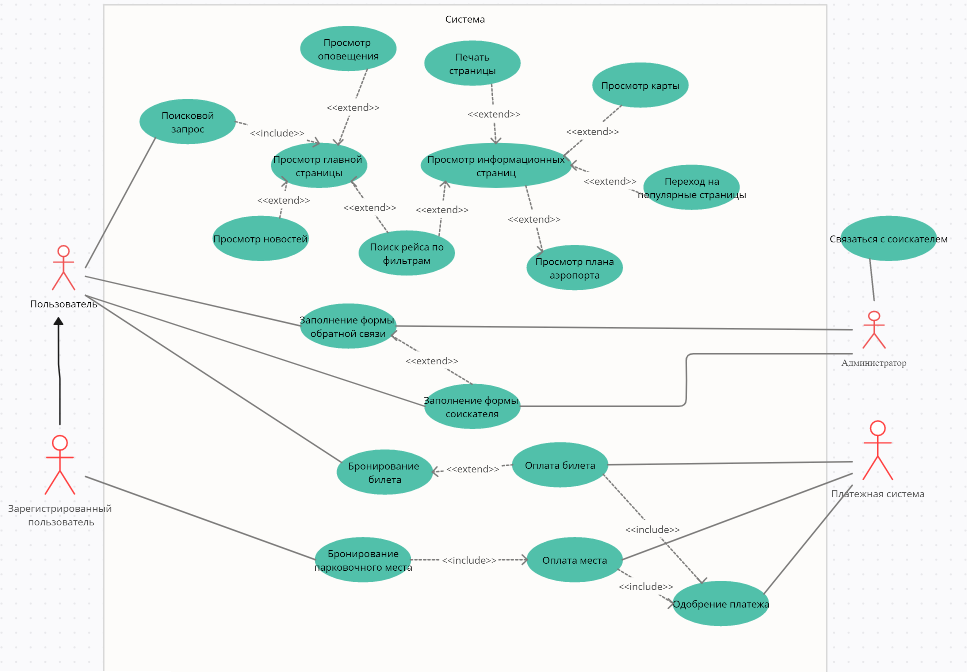
\includegraphics[width=\textwidth]{use-case-diagram/Use-case.png}
  \centering
\end{figure}

\section{Вывод}

Благодаря выполнению данной лабораторной работы, мы смогли поработать над описанием
процесса разработки по методологии RUP, а также смоделировали use-case диаграмму и 
описали прецеденты использования.
\end{document}